\documentclass[a4paper,12pt]{article}
\newtheorem{thm}{Theorem}
\setlength{\oddsidemargin}{0.25in}
\setlength{\textwidth}{6in}
\setlength{\topmargin}{-0.25in}
\setlength{\headheight}{0.3in}
\setlength{\headsep}{0.2in}
\setlength{\textheight}{9in}
%\setlength{\footskip}{0.1in}
\usepackage{multirow}
\usepackage{fullpage}
\usepackage{graphicx}
\usepackage{amsthm}
\usepackage{amssymb}
\usepackage{url}
\usepackage{algorithm}
\usepackage{algorithmic}
\usepackage{amsfonts}
\usepackage{mathtools}
\newcommand{\quotes}[1]{``#1''}

\usepackage{hyperref}
\hypersetup{
    colorlinks=true,
    linkcolor=blue,
    filecolor=magenta,      
    urlcolor=blue,
}

% ===== ===== ===== ===== ===== % 
% New commands set by Chuck Jia
% ===== ===== ===== ===== ===== % 

\newcommand{\code}[1]{\texttt{#1}}
\newcommand{\qnum}[1]{\noindent\textcolor{blue}{\textbf{(#1)}}}
\newcommand{\ds}{\displaystyle}
\newcommand{\tx}[1]{\text{#1}}
\newcommand{\ba}{\[\begin{aligned}}
\newcommand{\ea}{\end{aligned}\]}
\newcommand{\sep}{\begin{center}\textcolor{gray}{\rule{\textwidth}{0.75pt}}\end{center}}
\usepackage{minted}
\usepackage{color}
\usepackage{xcolor}
\definecolor{myorange}{RGB}{255, 165, 0}
\definecolor{mydarkgreen}{RGB}{0, 100, 0}
\definecolor{mybrickred}{RGB}{132, 31, 39}
\definecolor{myfirebrick}{RGB}{178, 34, 34}

\begin{document}
\title{Homework 3\\ Applied Machine Learning \\ Fall 2017\\ CSCI-P 556/INFO-I 526}         % Enter your title between curly braces
\author{Chuck Jia}        % Enter your name between curly braces
\date{\today}          % Enter your date or \today between curly braces
\maketitle
\makeatother     % `@' is restored as a "non-letter" character
\pagestyle{plain}
\section*{Directions}
Please follow the syllabus guidelines in turning in your homework.  I am providing the \LaTeX{} of this document too. This homework is due Friday Oct 27, 2017 11:59p.m. \textbf{OBSERVE THE  TIME}. Absolutely no homework will be accepted after that time. Bring a hard-copy to Tuesday's class on the 1st.
If you do not bring a hard-copy with the statement of your own work, the homework will not be
accepted.  All the work should be your own.  Within a week, AIs can contact students to examine code; students must meet within three days.  The session will last no longer than 5 minutes.  If the code does not work, the grade for the program may be reduced.  Lastly, source code cannot be
 modified post due date.
 

 %%%%%%%%%%%%%%%%%%%%%%%%%%%%%%%%%%%%%%%%%%%%%%%%%%%%%
 
 
\section*{Linear  and Logistic Regression} 
This part is provided to help you implement linear and logistic regression.

\subsection*{Notations} 


\begin{itemize}
\item $\Delta$: data set
\item $m$: number of training examples, $n$: number of features, $x$'s:  input variables, $y$'s:  output variable.
\item     $(x^{(i)}, y^{(i)}): i^{th}$ training example
\item $x^{(i)}_j$: value of feature $j$ in $i^{th}$ training example
\item $x_0 = 1$ (the first feature ($x_0$) is a vector of $1$'s) -- you should add  $x_0 = 1$  to data before answering the questions.
\item  $\alpha$: learning rate 
\end{itemize}


\subsection*{Linear Regression} 

\begin{itemize}
\item[] \textbf{Parameters:} $ {\theta} = (\theta_0,\ldots,\theta_n) $
\item[] \textbf{Hypothesis/Model:} $ h_{\theta}(x) = \theta(x) = \theta^Tx = \theta_0 x_0+\ldots+\theta_n x_n $
\item[] \textbf{Cost Function:} $J(\theta_0,\ldots,\theta_n) = \frac{1}{2m} \sum_{i=1}^{m} (h_{\theta}(x^{(i)})-y^{(i)})^2$
\item[]\ \ \ \ \ \ \ \ \  \  \ \ \ \ \ \ \ \ \ \ \ \  \ \   $\Rightarrow   \frac{\partial }{\partial \theta_j } J(\theta_0,\ldots,\theta_n)  = \frac{1}{m}  \sum_{i=1}^{m} (h_{\theta}(x^{(i)})-y^{(i)}) \ x_j^{(i)} $
\end{itemize}


\subsection*{Logistic Regression} 
\begin{itemize}
\item[] \textbf{Parameters:} $ {\theta} = (\theta_0,\ldots,\theta_n) $
\item[] \textbf{Hypothesis/Model:} $ h_{\theta}(x) =\frac{1}{1+ e^{-\theta^Tx}} $
\item[] \textbf{Cost Function:} $J(\theta_0,\ldots,\theta_n) = \frac{1}{m}\big[-y^{(i)}\ log(h_{\theta}(x^{(i)}))-(1-y^{(i)})\ log(1-h_{\theta}(x^{(i)}))\big]$
\item[]\ \ \ \ \ \ \ \ \  \  \ \ \ \ \ \ \ \ \ \ \ \  \ \   $\Rightarrow   \frac{\partial }{\partial \theta_j } J(\theta_0,\ldots,\theta_n)  = \frac{1}{m}  \sum_{i=1}^{m} (h_{\theta}(x^{(i)})-y^{(i)}) \ x_j^{(i)} $
\end{itemize}

  
 
\subsection*{Linear Regression and Logistic Regression via Gradient Descent} 

\textbf{Repeat until convergence}\big\{
  $$ \theta_j \leftarrow  \theta_j -\alpha \frac{1}{m}  \sum_{i=1}^{m} h_{\theta}(x^{(i)})-y^{(i)}) \ x_j^{(i)}     $$ \big\}
   (simultaneously update $\theta_j$ for all $j$)






  %%%%%%%%%%%%%%%%%%%%%%%%%%%%%%%%%%%%%%%%%%%%%%%%%%%%%

                                   %     PROBLEM 1

 %%%%%%%%%%%%%%%%%%%%%%%%%%%%%%%%%%%%%%%%%%%%%%%%%%%%%
 
\newpage
\section*{Problem 1 [100 points]} 

Implement gradient descent algorithm for linear regression and answer the following questions. In this question, you are asked to use your gradient descent implementation to fit linear models to Auto data set which can be found in the \quotes{ISLR} package.

\begin{verbatim}
> require("ISLR")
> Auto
\end{verbatim}

\subsubsection*{Initialization of the parameters} 

\begin{itemize}
\item Add $x_0 =1$ to  data (all ones feature)
\item Set the learning rate $\alpha$ to 0.01 and iteration number to 1000. You may need to use different $\alpha$ and iteration number values if you observe they are  not sufficient.
\item Initialize $\theta$'s as $0$'s -- $(\theta_0,\ldots, \theta_n) = (0,\ldots,0)$
\end{itemize}



\subsection*{Simple Linear Regression  [45 points]} 

\begin{enumerate}
  \item[\textbf{1.1}] Perform a simple linear regression with \quotes{mpg} as the response and  \quotes{horsepower} as the predictor. What are the parameters $\theta = (\theta_0,\theta_1)$? Is the relationship between horsepower and mpg positive or negative?   [20 pt]
   \item[\textbf{1.2}] Plot the output variable and the input variable. Display the least squares regression line.   [5 pt]
  \item[\textbf{1.3}] Use the model obtained in Q.1.1 to make predictions. What is the "mpg" value for \quotes{horsepower $= 220$}?  [5 pt]
 \item[\textbf{1.4}] In a contour plot,  show how $J(\theta$) varies with changes in $\theta_0$ and $\theta_1$. Does $J(\theta)$ have a global minimum?  [10 pt]
 \item[\textbf{1.5}] The closed-form solution to linear regression is $\theta = (\Delta^T\Delta)^{-1} \Delta^Ty$. Report the coefficients using this formula.  [5 pt]
\end{enumerate}


\subsection*{ Multivariate Linear Regression  [55 points]} 



\begin{enumerate}
  \item[\textbf{1.6}] First, perform feature scaling (mean normalization) over the Auto data set to make gradient descent converge faster. Then, train a multivariate linear regression with \quotes{mpg} as the response and  all other variables  except name as the predictors.  Report the parameters ($\theta$'s). What does the coefficient for the \quotes{year} variable suggest? [30 pt]
  \item[\textbf{1.7}]   Use the model obtained in Q.1.6 to make predictions. What is the \quotes{mpg} value for $(x_1,\ldots,x_7) =  (4,300,200,3500,11,70,2)$?  [5 pt]
\item[\textbf{1.8}]In this question, you are asked to test different learning rates. Run your gradient descent for 100 iterations at the chosen learning rates $(\alpha_1 = 3,  \alpha_2 = 0.3, \alpha_3 = 0.03,   \alpha_4 = 0.00003)$. For each learning rate, make a plot that shows how $J(\theta$) changes at each iteration. Discuss the plots? i.e., which one looks better? does it converge? [15pt]
\item[\textbf{1.9}] Calculate the  coefficients using the normal equations. [5pt]
\end{enumerate}

\sep 

\noindent\textcolor{blue}{\textbf{Simple Linear Regression}}\bigskip 

\qnum{1.1}
The linear regression is performed by commands in \code{Prob1-Q1.R}. To run the file, execute all commands in the file directly, or execute the command in the first part of the file \code{Prob1-Part1-SimpleLR.R}.

The result of the regression is 
\[
    \hat\theta = (\hat\theta_0, \hat\theta_1)^T
    = (39.93586, -0.1578447)^T
\]

From this, we can see that the relationship between horsepower and mpg is negative, because the slope $\hat\theta_1 = -0.1578447$ is negative.
\bigskip




\qnum{1.2}
\begin{center}
    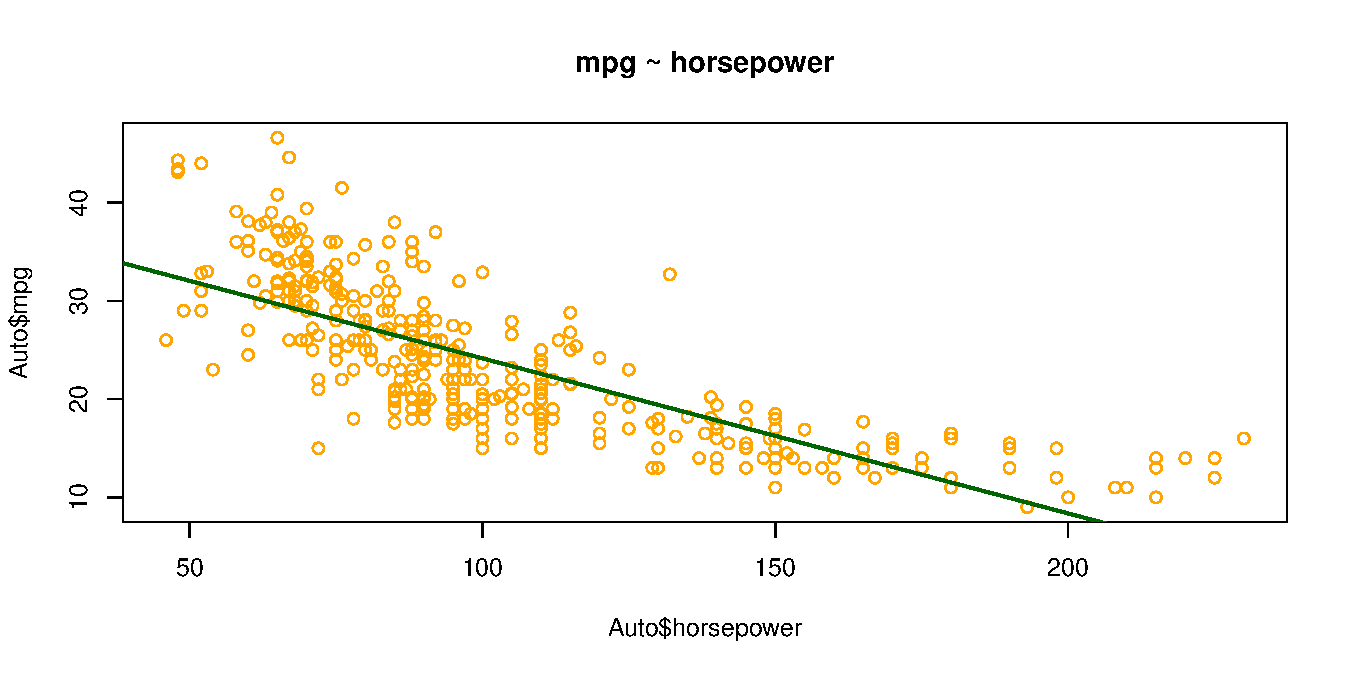
\includegraphics[width=0.9\linewidth]{Images/Prob1-2.pdf}
  
    % Comments
    \parbox{0.9\textwidth}{\textit{
    In the plot, the \textcolor{mydarkgreen}{green line} represents the least squares regression line.
    }}
\end{center}


\qnum{1.3}
Using the model obtained in Q.1.1, when horsepower = 220,
\[
    \hat{\tx{mpg}} = \hat\theta_0 + \hat\theta_1\times 220
    = 39.93586 -0.1578447 \times 220
    = 5.210026
\]






\qnum{1.4}
The contour plot is shown below
\begin{center}
    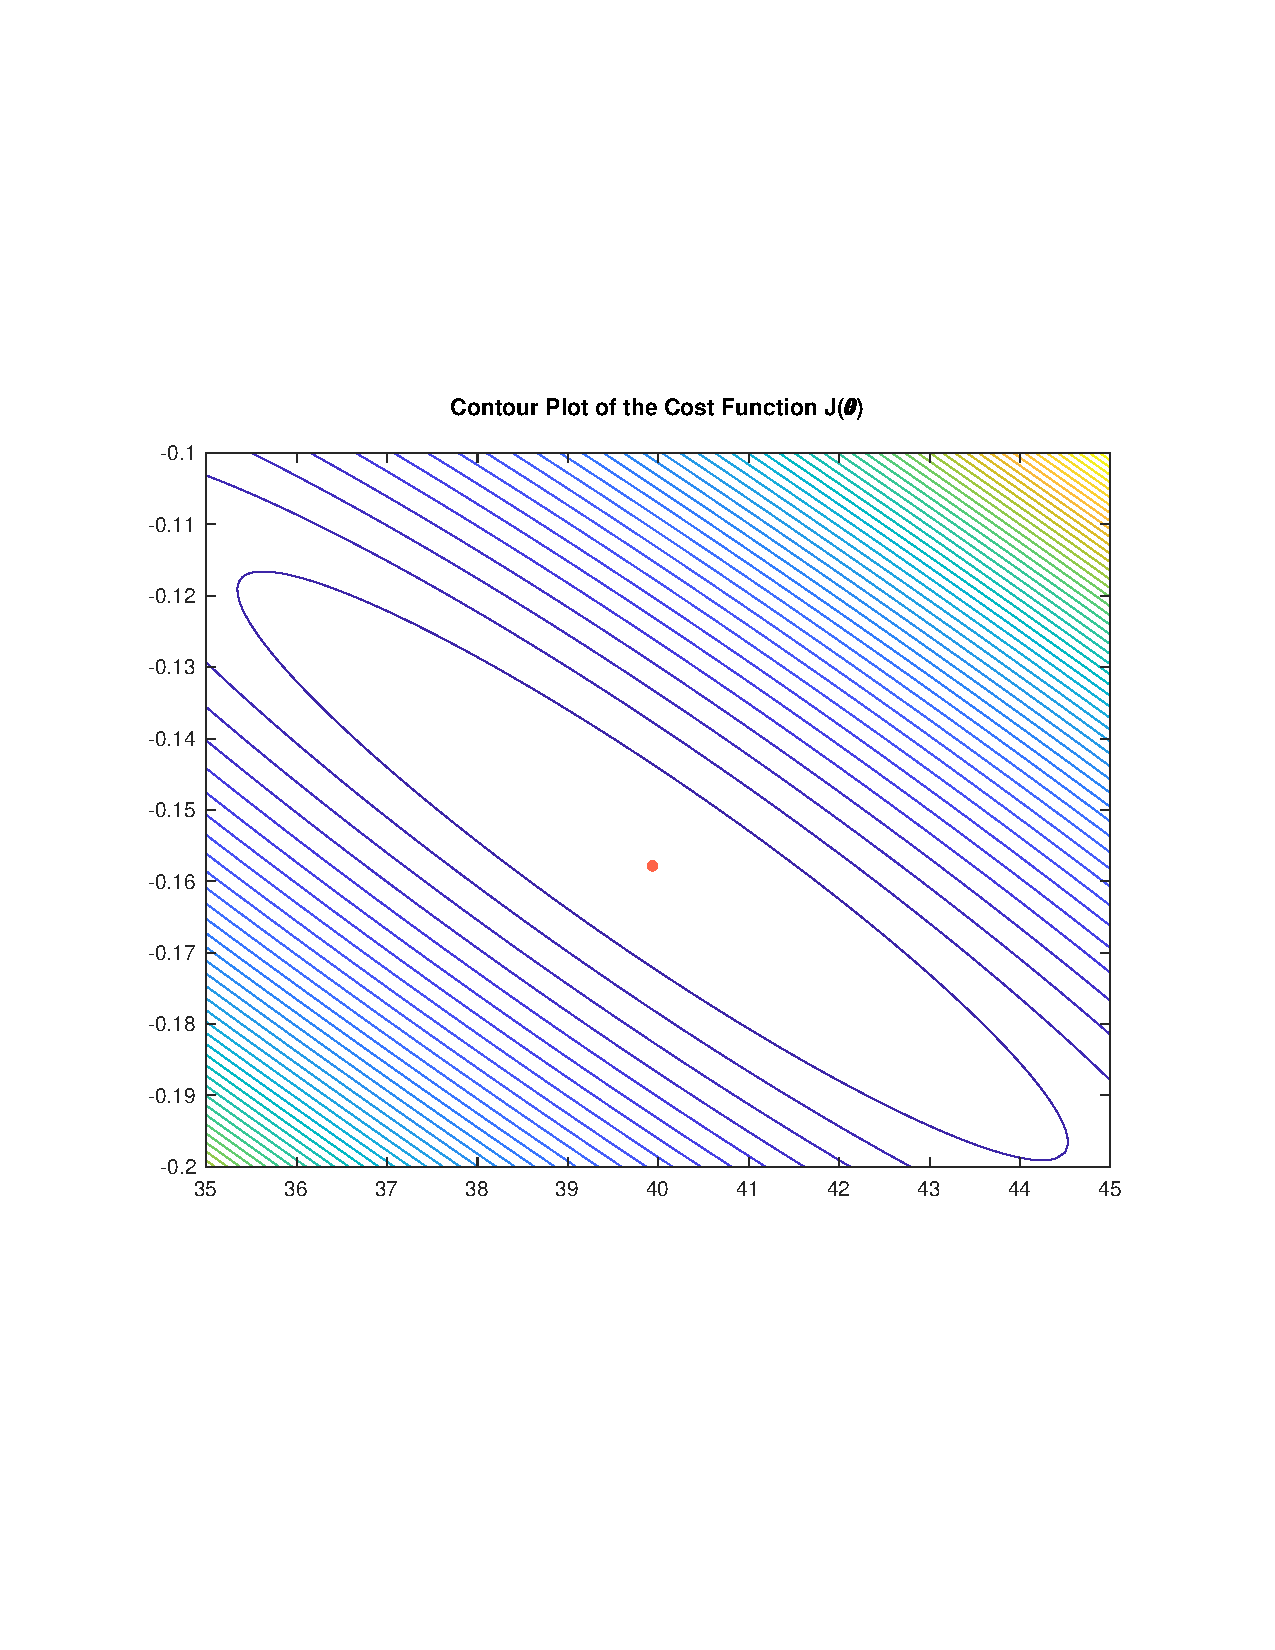
\includegraphics[width=0.9\linewidth, trim={0 6.5cm 0 6cm}]{Images/Prob1-4-Contour.pdf}
  
    % Comments
    \parbox{0.65\textwidth}{\textit{In the plot, the \textcolor{myorange}{orange dot} in the middle represents the solution from the gradient descent method. The transition of level curve color from yellow to purple represents the descending of the cost function $J(\theta)$.
    }}
\end{center}
\bigskip\bigskip

For convenience of analysis, we also provide a surface plot for the cost function.
\begin{center}
    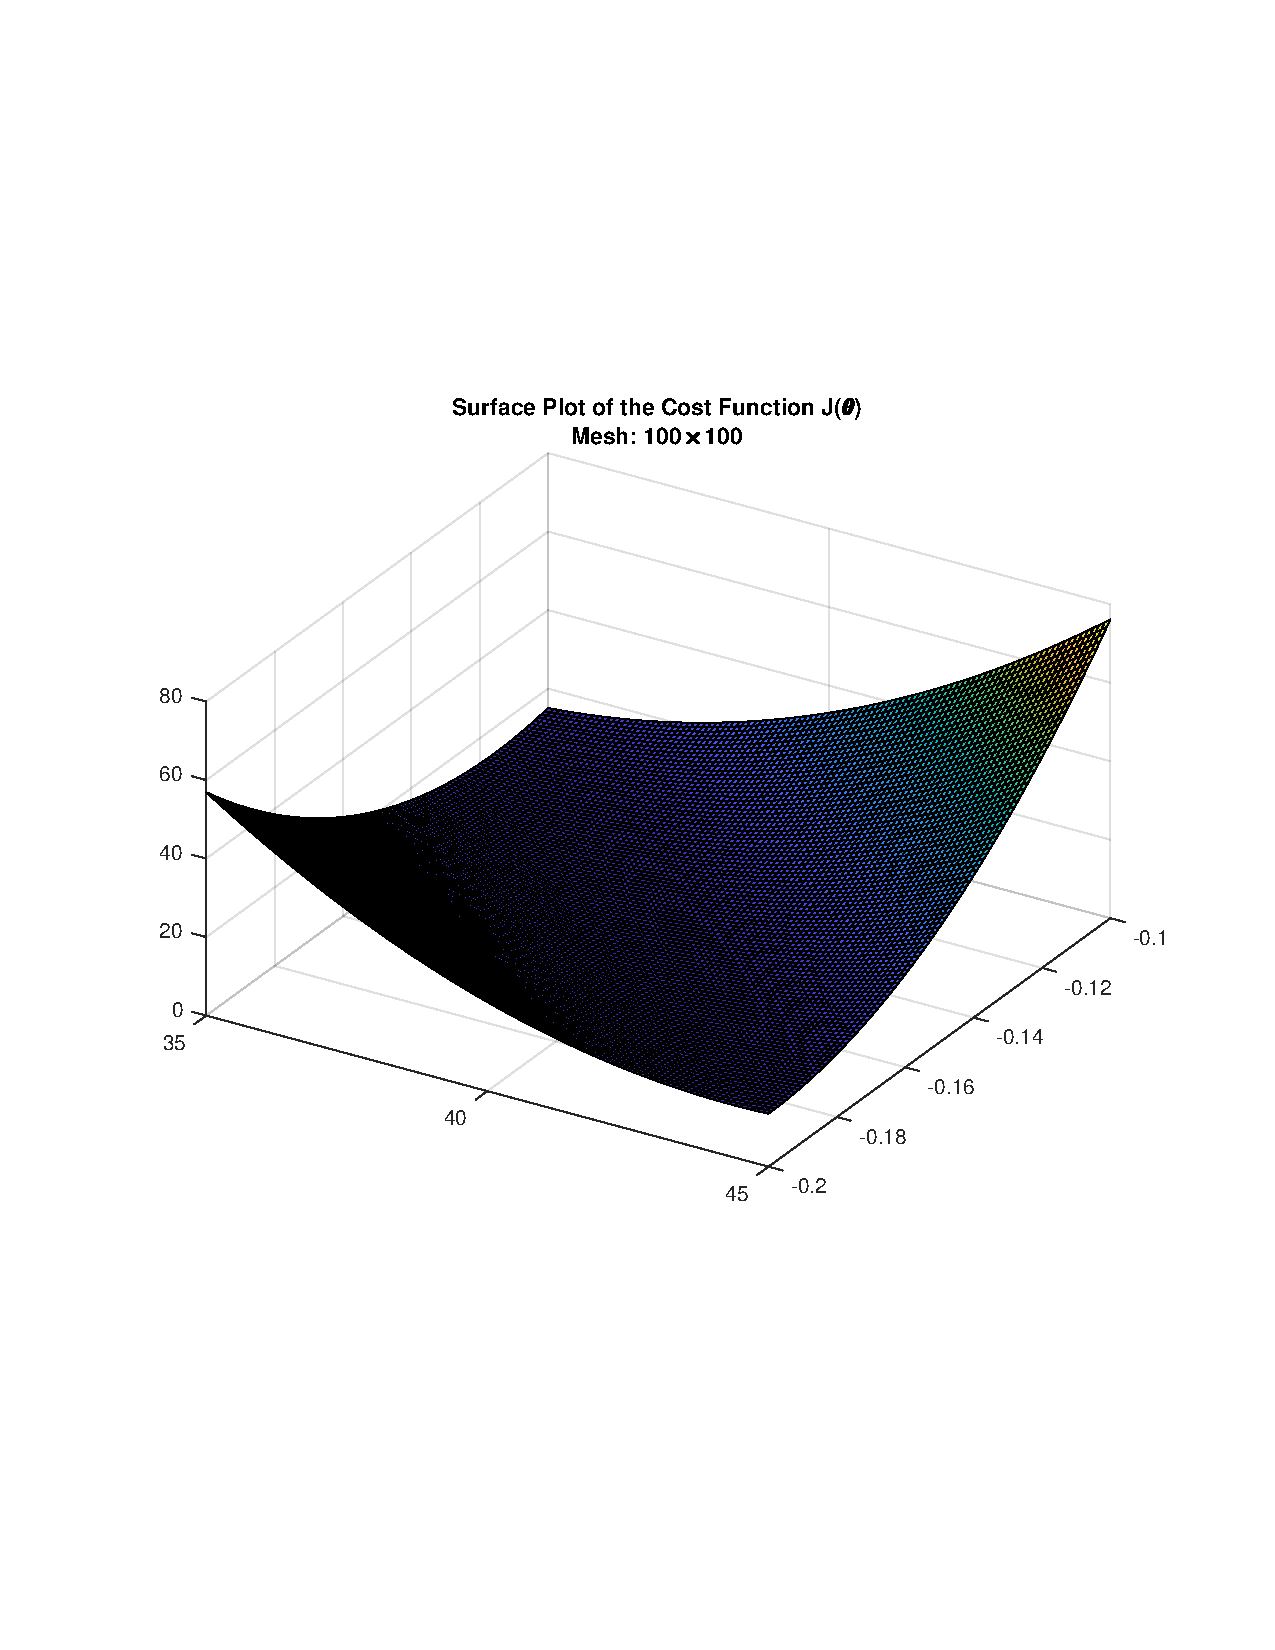
\includegraphics[width=0.9\linewidth, trim={0 6.5cm 0 6cm}]{Images/Prob1-4-Surf.pdf}
\end{center}
\bigskip



\qnum{1.5}
The result calculated by the closed form formula is
\[
    \hat\theta = (\hat\theta_0, \hat\theta_1)^T
    = (39.93586, -0.1578447)^T
\]
\bigskip


\noindent\textcolor{blue}{\textbf{Multivariate Linear Regression}}\bigskip  

\qnum{1.6}
The parameters in the result of the gradient descent solver of the linear regression is 
\ba 
    \hat\theta = (\hat\theta_0, \hat\theta_1, \hat\theta_2, \cdots, \hat\theta_7)^T
    = \begin{pmatrix}
    5.741574\times 10^{-16} \\
    -0.1078237 \\ 
    0.2667399 \\ 
    -0.08359488 \\ 
    -0.704555 \\ 
    0.02848128 \\ 
    0.3543428 \\ 
    0.1471847
    \end{pmatrix}
\ea 

In \code{R}, the result with the corresponding labels is 
\begin{verbatim}
                      [,1]
Intercept     5.741574e-16
cylinders    -1.078237e-01
displacement  2.667399e-01
horsepower   -8.359488e-02
weight       -7.045550e-01
acceleration  2.848128e-02
year          3.543428e-01
origin        1.471847e-01
\end{verbatim}

The coefficient for ``year" $\theta_{\tx{year}}$ is 0.3543428. It represents the ``slope" along the feature ``year" direction of the regression affine hyperplane. It shows how fast the mpg value would increase when the year value increases. In other words, it is the correlation between mpg and year in the regression model. It suggests that in the regression model we derived, the scaled mpg value would increase by 0.3543428, if the scaled feature ``year" increases its value by 1.

Moreover, if we scale back and use the original units, then this coefficient would suggest that if we increase the value of the feature ``year" by 1, the mpg would increase its value in the original unit by
\[
    \hat\theta_{\tx{year}}\sigma_{\tx{mpg}}\sigma_{\tx{year}}^{-1}
    = 0.7507725
\]
where $\sigma_{\tx{mpg}}$ and $\sigma_{\tx{year}}$ are the sample standard deviations of features ``mpg" and ``year" without scaling.
\bigskip



\qnum{1.7}
The scaled values for $x$ is 
\ba 
     & (x_1^{\tx{scaled}}, x_2^{\tx{scaled}},\ldots ,x_7^{\tx{scaled}})\\
    &= (  -0.8629108,    1.0090211,    2.4818845,    0.6150391,   -1.6460856, -1.6232409,   0.5257105)
\ea 
This is performed by subtracting each feature element by the original feature sample mean, and then dividing each feature element by the original feature sample standard deviation.

Using the formula, the predicted value of mpg is
\[
    \hat{\tx{mpg}}^{\tx{scaled}} =
    (1,x_1^{\tx{scaled}},\cdots,x_7^{\tx{scaled}})\hat\theta =  (1,x_1^{\tx{scaled}},\cdots,x_7^{\tx{scaled}})(\hat\theta_0, \hat\theta_1, \hat\theta_2, \cdots, \hat\theta_7)^T
    = -0.8233031
\]
Now scale back to the original unit, we have
\[
    \hat{\tx{mpg}} = \hat{\tx{mpg}}^{\tx{scaled}} \sigma_{\tx{mpg}} + \mu_{\tx{mpg}}
    = 17.02003
\]
$\sigma_{\tx{mpg}}$ and $\mu_{\tx{mpg}}$ are the sample standard deviation and sample mean of feature ``mpg" in its original unit without scaling.

The \code{R} code for the calculation of this question can be found in the Problem 1.7 part of the file \code{Prob1-Part2-MultiLR.R}.
\bigskip






\qnum{1.8}
\begin{center}
    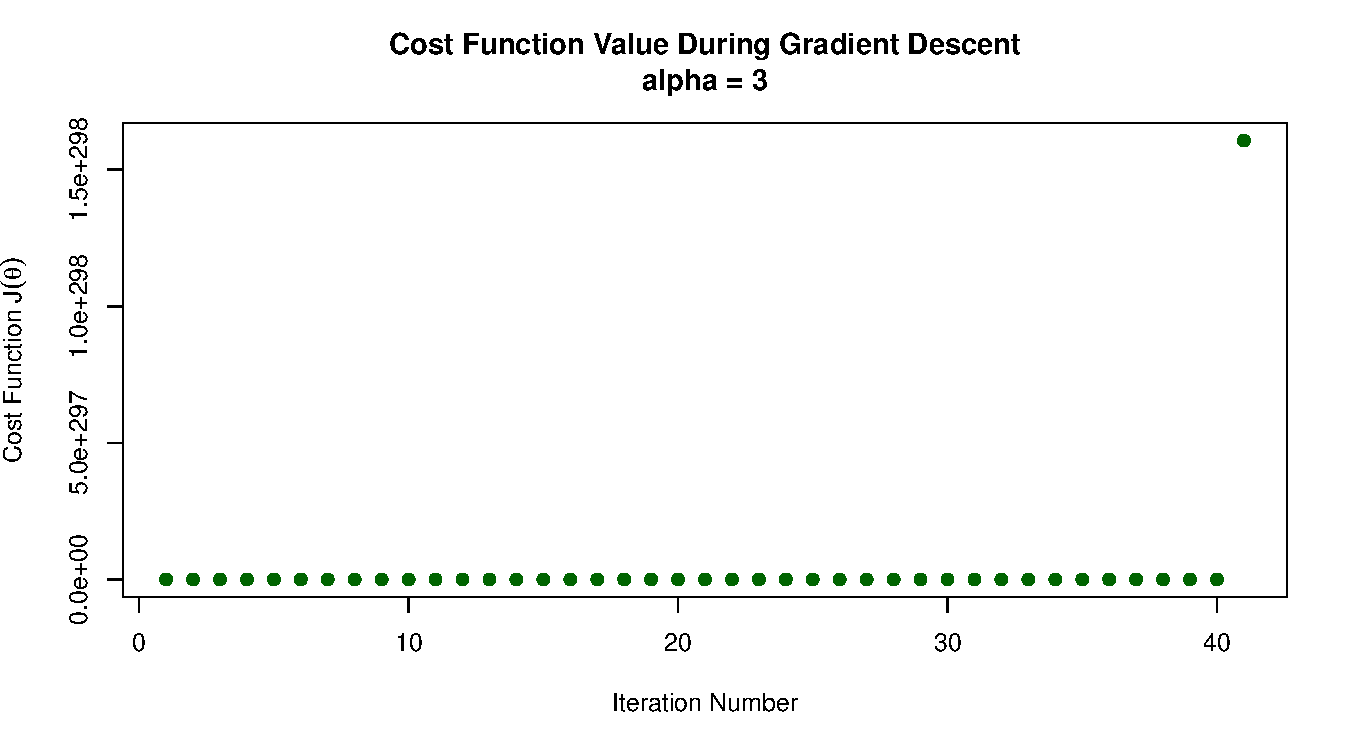
\includegraphics[width=0.9\linewidth]{Images/Prob1-8-alpha1.pdf}
    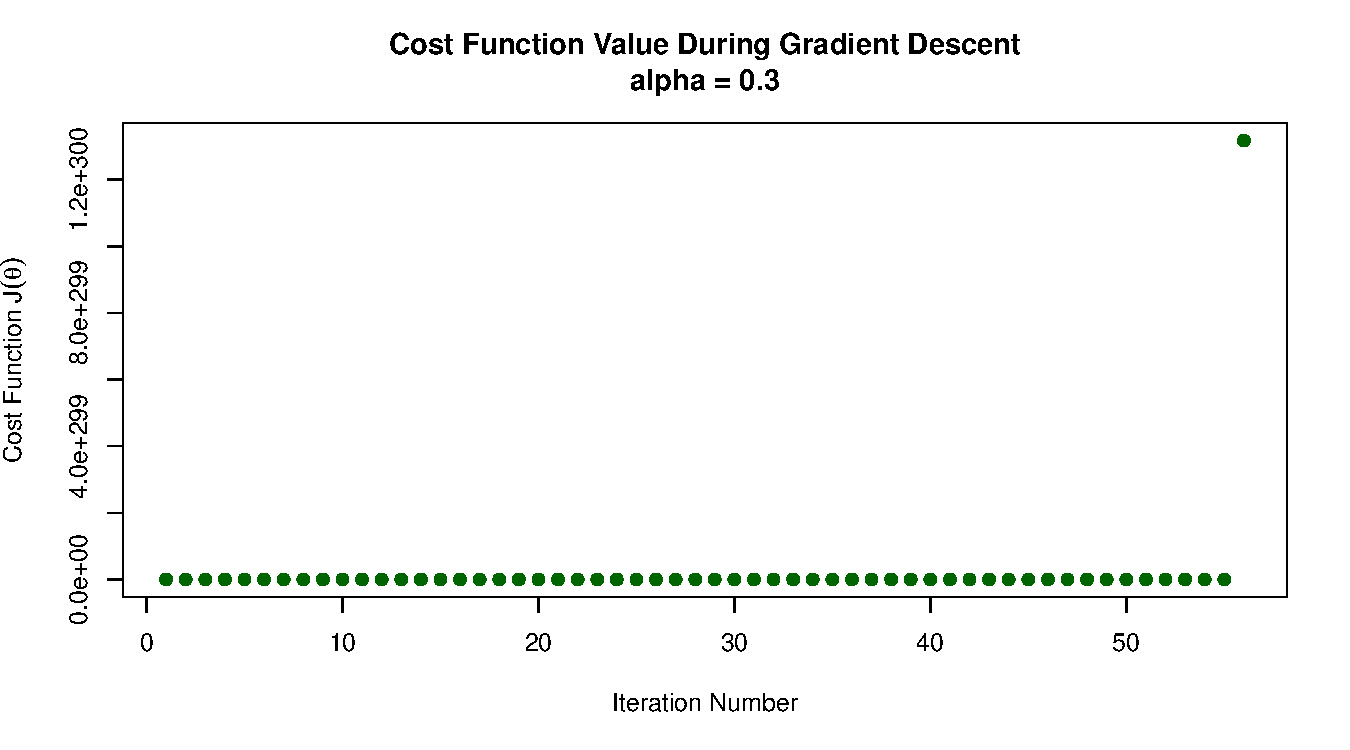
\includegraphics[width=0.9\linewidth]{Images/Prob1-8-alpha2.pdf}
    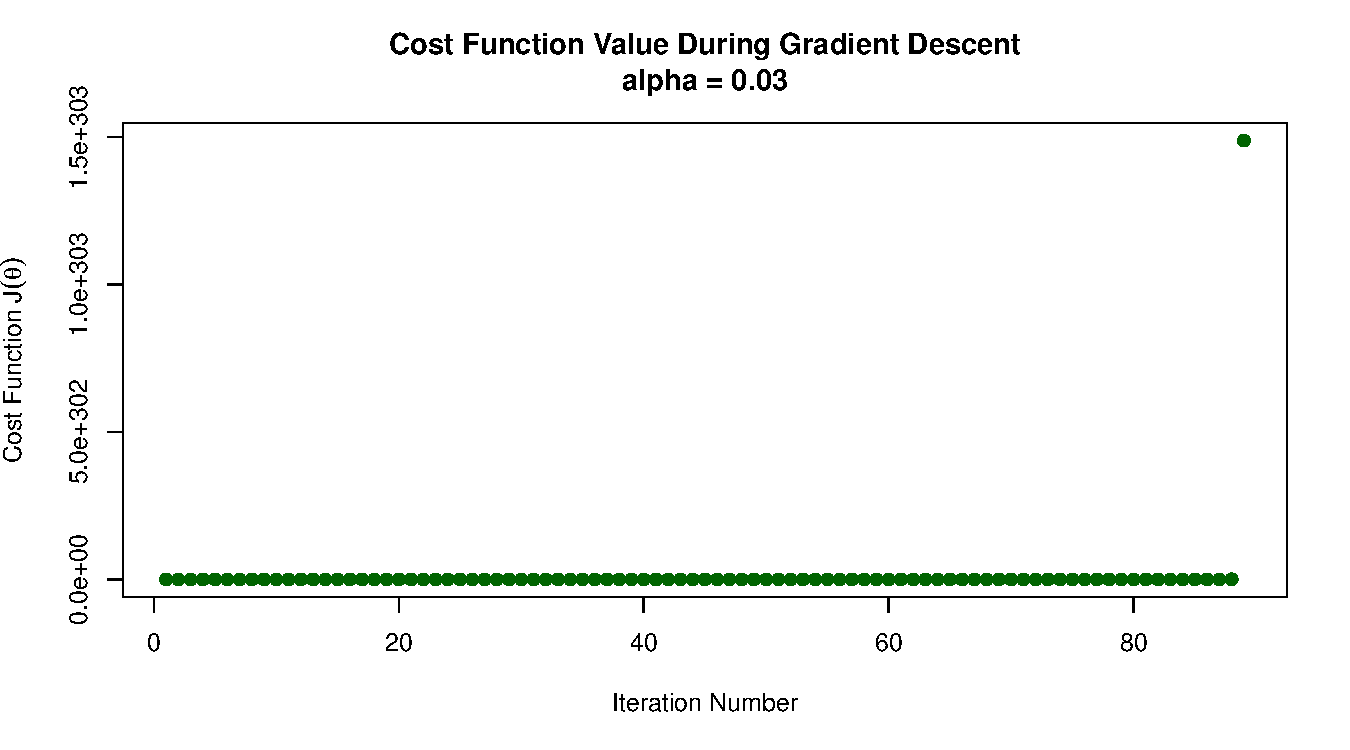
\includegraphics[width=0.9\linewidth]{Images/Prob1-8-alpha3.pdf}
    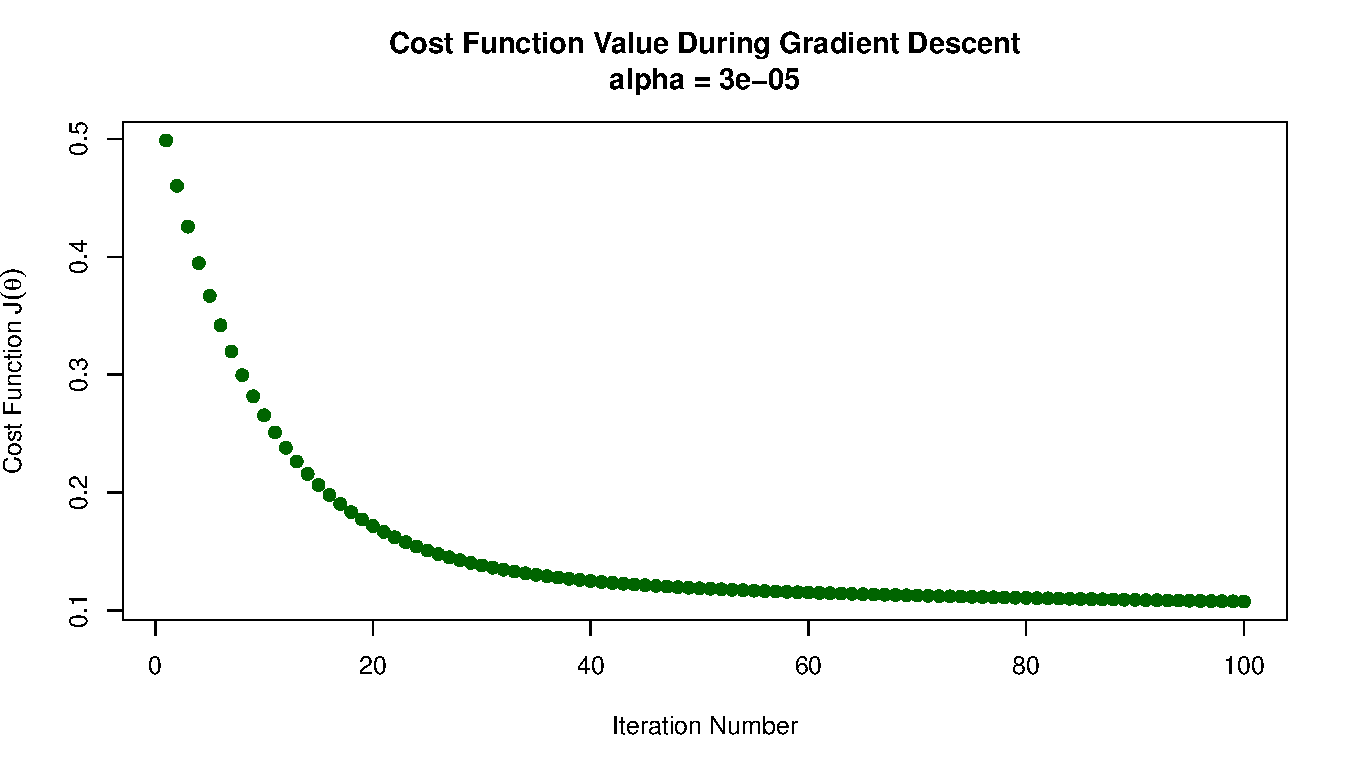
\includegraphics[width=0.9\linewidth]{Images/Prob1-8-alpha4-itr100.pdf}
\end{center}

\noindent\textcolor{blue}{\textbf{Analysis}}
\medskip

As we can see from the plots, when we use $\alpha = 3, 0.3,$ or $0.03$, the method does not converge and the cost function blows up. When $\alpha=0.00003$, from the fourth graph, we can see that the method converges. Therefore, the plot with $\alpha=0.00003$ looks much better than others.

Note that in the first 3 graphs, it seems that all cost function values, except the last one, are the same. This is not really the case. The cost function in fact grows at exponential rate, therefore masks the true growth rate in the plot. To show more clearly how fast the growth is, we provide below the log plots for the first 3 cases.



\begin{center}
    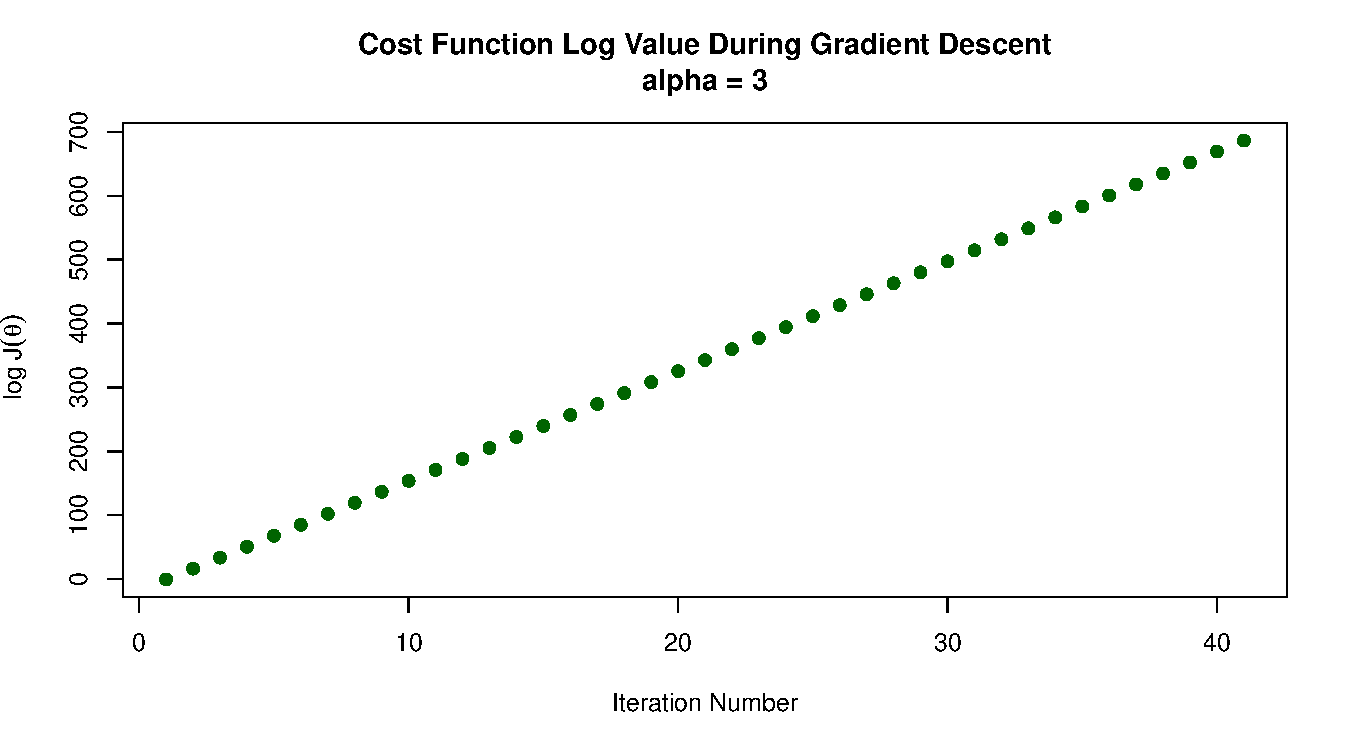
\includegraphics[width=0.9\linewidth]{Images/Prob1-8-alpha1-log.pdf}
    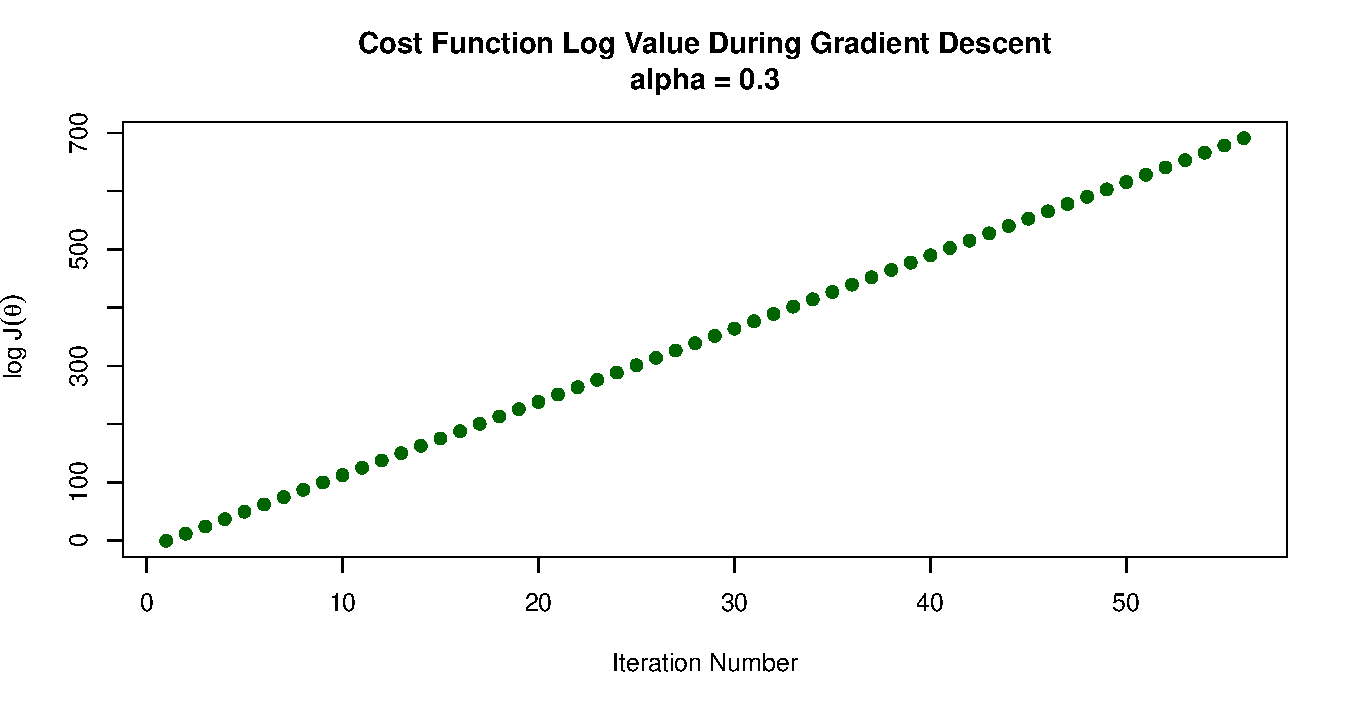
\includegraphics[width=0.9\linewidth]{Images/Prob1-8-alpha2-log.pdf}
    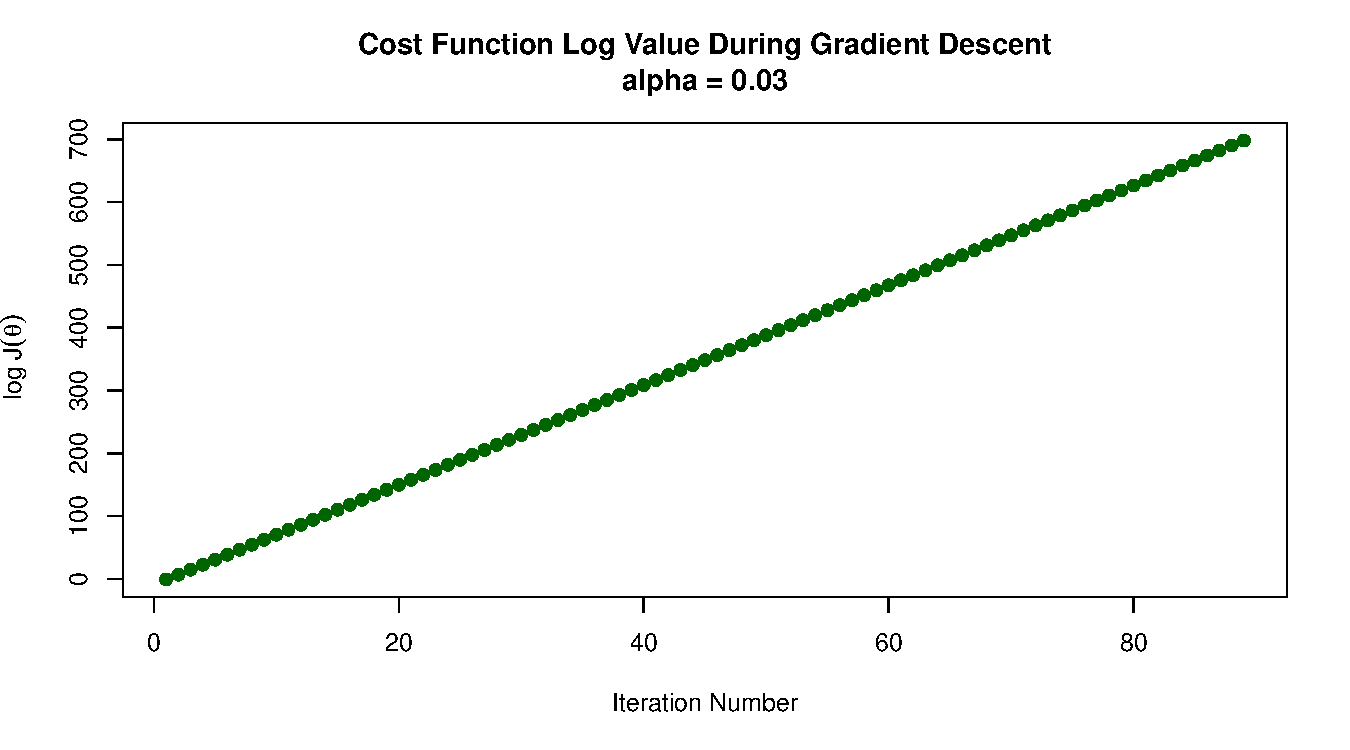
\includegraphics[width=0.9\linewidth]{Images/Prob1-8-alpha3-log.pdf}
\end{center}

Also, here we give a plot for $\alpha = 0.00003$ in the long run, until actual convergence.
\begin{center}
    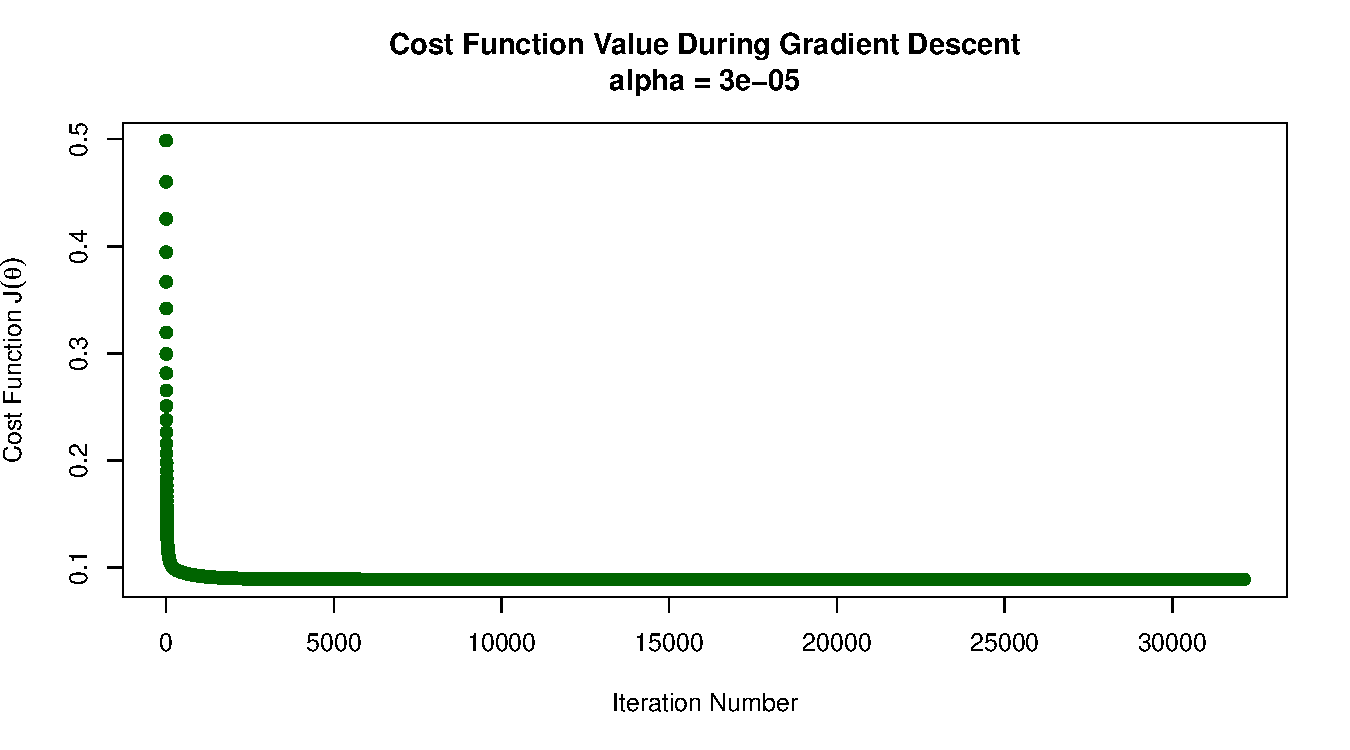
\includegraphics[width=0.9\linewidth]{Images/Prob1-8-alpha4.pdf}
\end{center}
\bigskip


\qnum{1.9}
By using the closed form formula,
\[
    \theta 
    = (X^TX)^{-1}X^Ty
    = \begin{pmatrix}
    -7.372575\times 10^{-16} \\
    -0.1078273 \\ 
    0.2667467 \\ 
    -0.08359632 \\ 
    -0.7045565 \\ 
    0.02848143 \\ 
    0.3543429 \\ 
    0.1471853
    \end{pmatrix}
\]
where $X\in\mathbb{R}^{m\times n}, y\in\mathbb{R}^{m}$ with 
\[
    X = \begin{pmatrix}
        x^{(1)}\\
        x^{(2)}\\
        \cdots\\
        x^{(m)}
    \end{pmatrix}
\]
being the matrix of sample values of the input variables, and $y$ being the vector of sample values of the response variable.

The result in \code{R} is given below, with the labels on the coefficients
\begin{verbatim}
Intercept    -7.372575e-17
cylinders    -1.078273e-01
displacement  2.667467e-01
horsepower   -8.359623e-02
weight       -7.045565e-01
acceleration  2.848143e-02
year          3.543429e-01
origin        1.471853e-01
\end{verbatim}

The actual calculation using the \code{R} language is performed in the "Problem 1.9" part of the file \code{Prob1-Part2-MultiLR.R}.





%%%%%%%%%%%%%%%%%%%%%%%%%%%%%%%%%%%%%%%%%%%%%%%%%%%%%
                                   %     PROBLEM 2

 %%%%%%%%%%%%%%%%%%%%%%%%%%%%%%%%%%%%%%%%%%%%%%%%%%%%%
 
\newpage
\section*{Problem 2 [35 points]} 

From textbook,  Chapter 3 exercises 13, 14  and 15 (Pages 124-126).
\sep 











\begin{center}
    \textcolor{myfirebrick}{\textbf{Exercise 13}}
\end{center}
\newcommand{\yr}{\textcolor{myfirebrick}{\code{y}} }
\newcommand{\xr}{\textcolor{myfirebrick}{\code{x}} }

\noindent\textcolor{blue}{\textbf{Original Noise}}\bigskip 

\qnum{a-c} 
The random data generation is performed in the \code{R} file \code{Prob2-Ex13-Part1.R}.

The length of the vector \yr is 100.
In the linear model, the coefficients are
\[
    \beta_0 = -1,\qquad 
    \beta_1 = 0.5
\]




\qnum{d} 
\begin{center}
    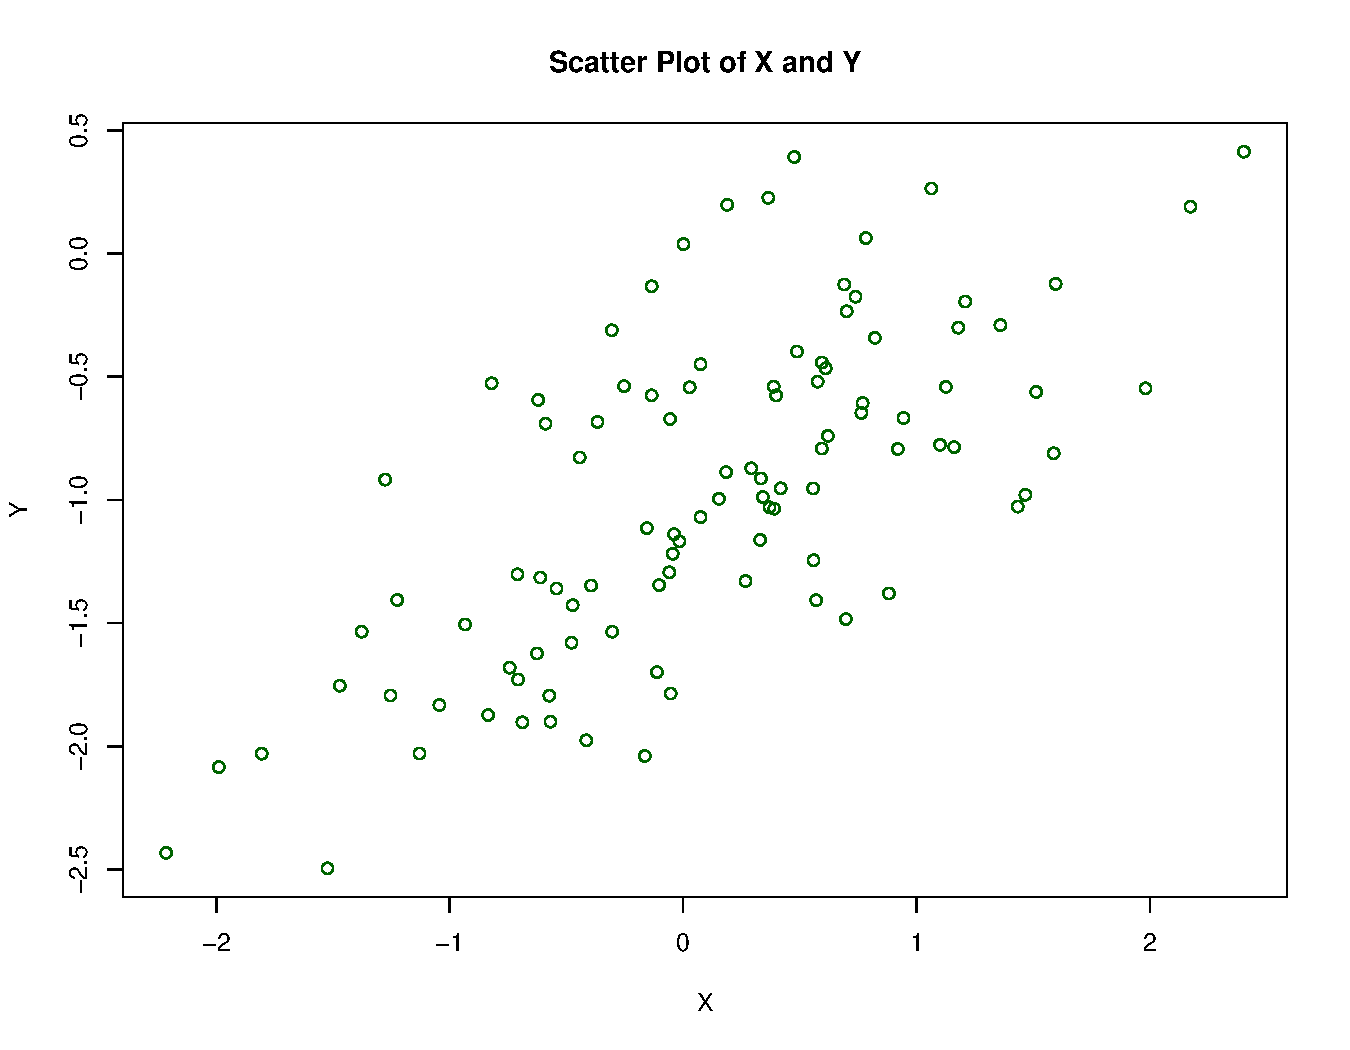
\includegraphics[width=0.9\linewidth]{Images/Prob2-Ex13-d.pdf}
\end{center}

The scatter plot shows that the \xr and \yr roughly has a linear correlation, but the relationship is very noisy as well.\bigskip


\qnum{e}
The linear fitting is performed in the \code{R} file \code{Prob2-Ex13-Part1.R}.
The coefficients in the results are
\[
    \hat\beta_0 = -1.0188463,\qquad 
    \hat\beta_1 = 0.4994698
\]
That is, our linear model can be described as 
\[
    \yr \sim \hat\beta_0 + \hat\beta_1\xr 
    = -1.0188463 + 0.4994698\xr
\]
This model is very close to the original population model without noise $Y = -1 + 0.5X$.

Comparing with the original $\beta_0$ and $\beta_1$, we calculate in \code{R}
\[
    |\hat\beta_0 - \beta_0| = 0.01884631 \quad 
    |\hat\beta_1 - \beta_1| = 0.0005301931
\]
We can see that our estimated coefficients $\hat\beta_0$, $\hat\beta_1$ are close to the population values $\beta_0$ and $\beta_1$. The difference is caused by the random noise $\epsilon$. 
Also we can see that $\hat\beta_1$ is very close to $\beta_1$. This is expected, as our random noise $\epsilon$ is symmetrical, i.e. with mean 0.
\bigskip


\qnum{f}
\begin{center}
    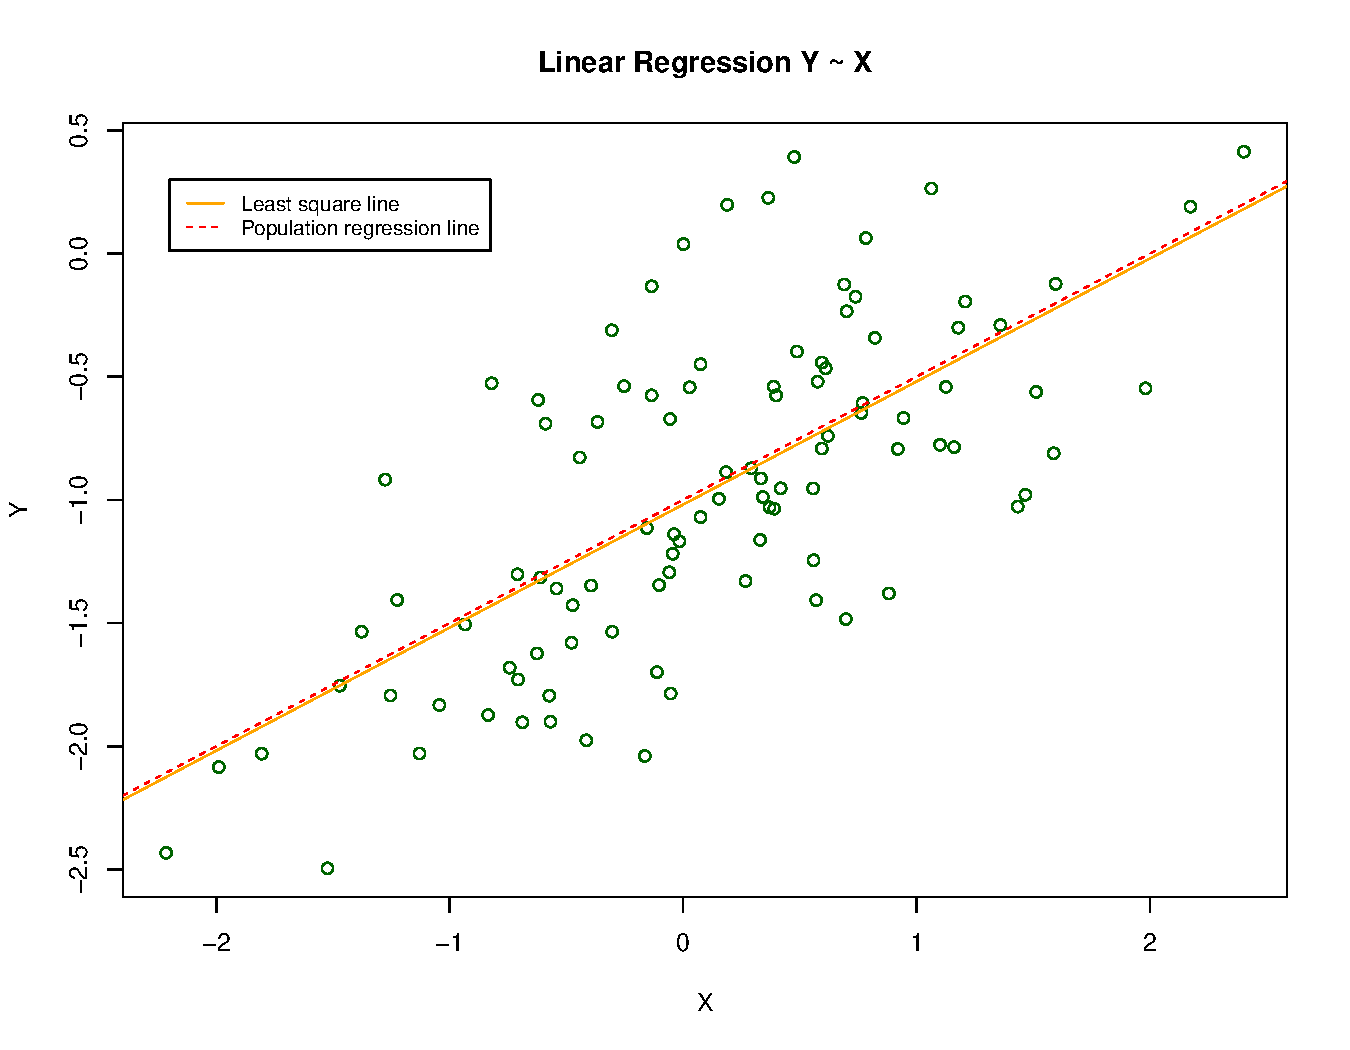
\includegraphics[width=0.9\linewidth]{Images/Prob2-Ex13-f.pdf}
    
    % Comments
    \parbox{0.65\textwidth}{\textit{In the plot, the \textcolor{myorange}{orange line} represents the least square line. The \textcolor{red}{red dotted line} represents the population regression line. The two lines are very close. Thus we chose dotted line for the population line to differentiate it from the other line.
    }}
\end{center}
\bigskip




\qnum{g}
Using commands in the \code{R} file \code{Prob2-Ex13-Part1.R}, we have the following result for the polynomial fitting 
\begin{verbatim}
(Intercept)           x      I(x^2) 
 -0.9716425   0.5085804  -0.0594606 
\end{verbatim}
or 
\[
    \yr \sim \hat{\beta}_0 + \hat{\beta}_1\xr + \hat{\beta}_2 \xr^2
    =
    -0.9716425
    + 0.5085804 \xr 
    -0.0594606 \xr^2 
\]

\newcommand{\rss}{\tx{RSS} }

In order to compare the result with the linear regression, we calculate the residual sum of squares (RSS) for both cases.
\ba 
    \rss_{\tx{linear}} = 22.7089,\qquad 
    \rss_{\tx{quadratic}} = 22.25728
\ea 
From the \rss point of view, the quadratic fitting performs better than the linear fitting, but the differences is not significant.
\bigskip\bigskip










\noindent\textcolor{blue}{\textbf{Less Noise}}\bigskip  

\qnum{h}
We use the noise $\epsilon\sim N(0, 0.2^2)$.

(a-c)
The length of the vector \yr is 100.
In the linear model, the coefficients are still
\[
    \beta_0 = -1,\qquad 
    \beta_1 = 0.5
\]

(d) 
\begin{center}
    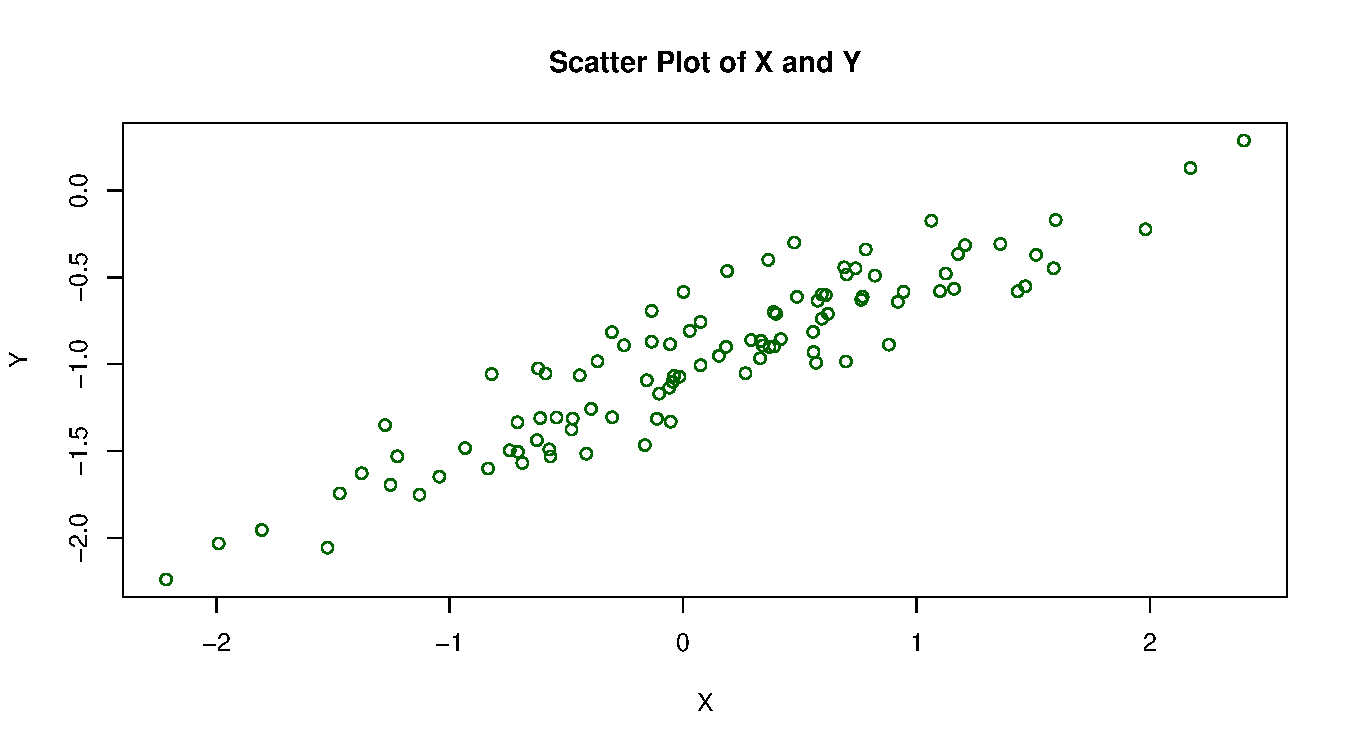
\includegraphics[width=0.9\linewidth]{Images/Prob2-Ex13-h-d.pdf}
\end{center}

The scatter plot shows that the \xr and \yr roughly has a linear correlation. The relationship is noisy, but the noise is smaller in scale compare to the original data set.
\bigskip



(e)
The coefficients in the results are
\[
    \hat\beta_0 = -1.0075385,\qquad 
    \hat\beta_1 = 0.4997879
\]
That is, our linear model can be described as 
\[
    \yr \sim \hat\beta_0 + \hat\beta_1\xr 
    = -1.0075385 + 0.4997879\xr
\]
This model is very close to the original population model without noise $Y = -1 + 0.5X$.

Comparing with the original $\beta_0$ and $\beta_1$, we calculate in \code{R}
\[
    |\hat\beta_0 - \beta_0| = 0.007538523 \quad 
    |\hat\beta_1 - \beta_1| = 0.0002120772
\]
We can see that our estimated coefficients $\hat\beta_0$, $\hat\beta_1$ are close to the population values $\beta_0$ and $\beta_1$. The difference is caused by the random noise $\epsilon$. 
Also we can see that $\hat\beta_1$ is very close to $\beta_1$. This is expected, as our random noise $\epsilon$ is symmetrical, i.e. with mean 0.
\bigskip




(f)
\begin{center}
    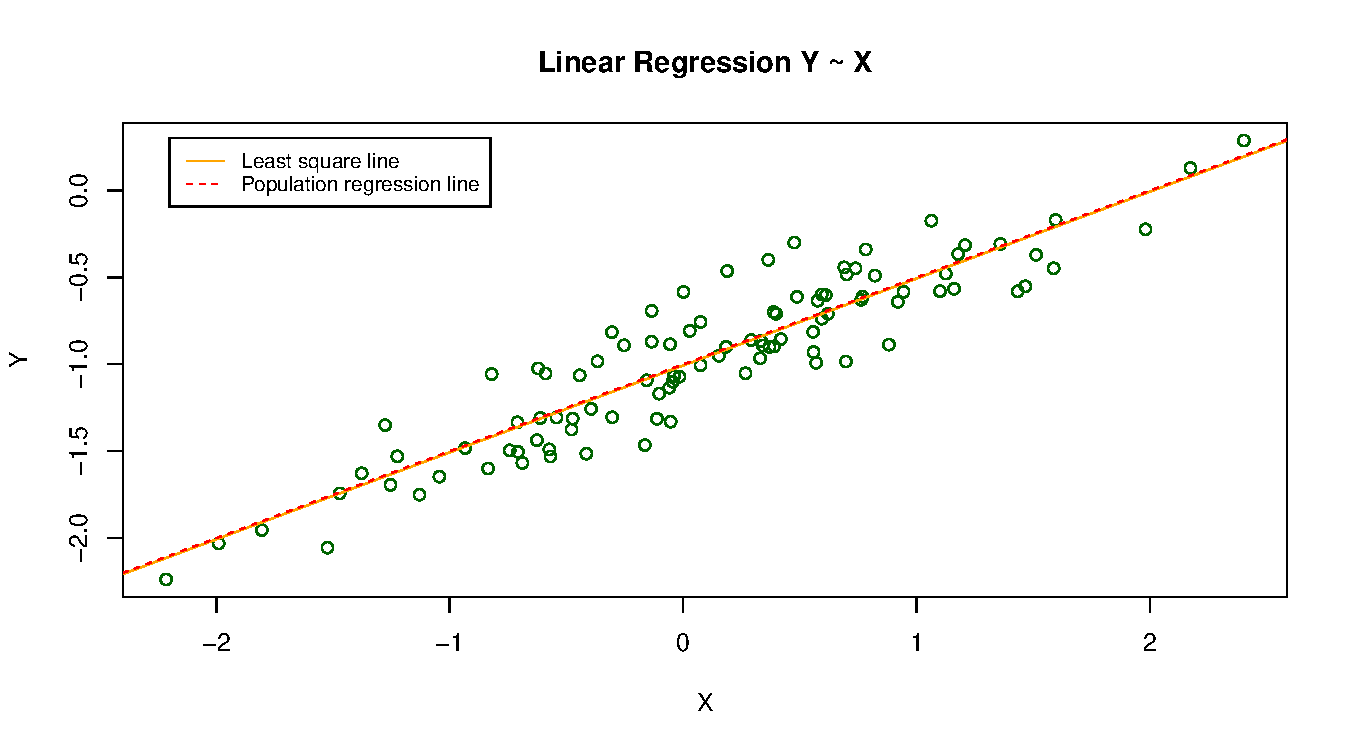
\includegraphics[width=0.9\linewidth]{Images/Prob2-Ex13-h-f.pdf}
    
    % Comments
    \parbox{0.65\textwidth}{\textit{In the plot, the \textcolor{myorange}{orange line} represents the least square line. The \textcolor{red}{red dotted line} represents the population regression line. The two lines are very close. Thus we chose dotted line for the population line to differentiate it from the other line.
    }}
\end{center}
\bigskip




(g)
Using commands in the \code{R} file \code{Prob2-Ex13-Part1.R}, we have the following result for the polynomial fitting 
\begin{verbatim}
(Intercept)           x      I(x^2) 
-0.98865700  0.50343217 -0.02378424  
\end{verbatim}
or 
\[
    \yr \sim \hat{\beta}_0 + \hat{\beta}_1\xr + \hat{\beta}_2 \xr^2
    =
    -0.98865700
    + 0.50343217 \xr 
    -0.02378424 \xr^2 
\]

In order to compare the result with the linear regression, we calculate the residual sum of squares (RSS) for both cases.
\ba 
    \rss_{\tx{linear}} = 3.633424,\qquad 
    \rss_{\tx{quadratic}} = 3.561164
\ea 
From the \rss point of view, the quadratic fitting performs better than the linear fitting, but the difference is not significant.
\bigskip\bigskip



































\noindent\textcolor{blue}{\textbf{More Noise}}\bigskip  

\qnum{i}
We use the noise $\epsilon\sim N(0, 0.7^2)$.

(a-c)
The length of the vector \yr is 100.
In the linear model, the coefficients are still
\[
    \beta_0 = -1,\qquad 
    \beta_1 = 0.5
\]

(d) 
\begin{center}
    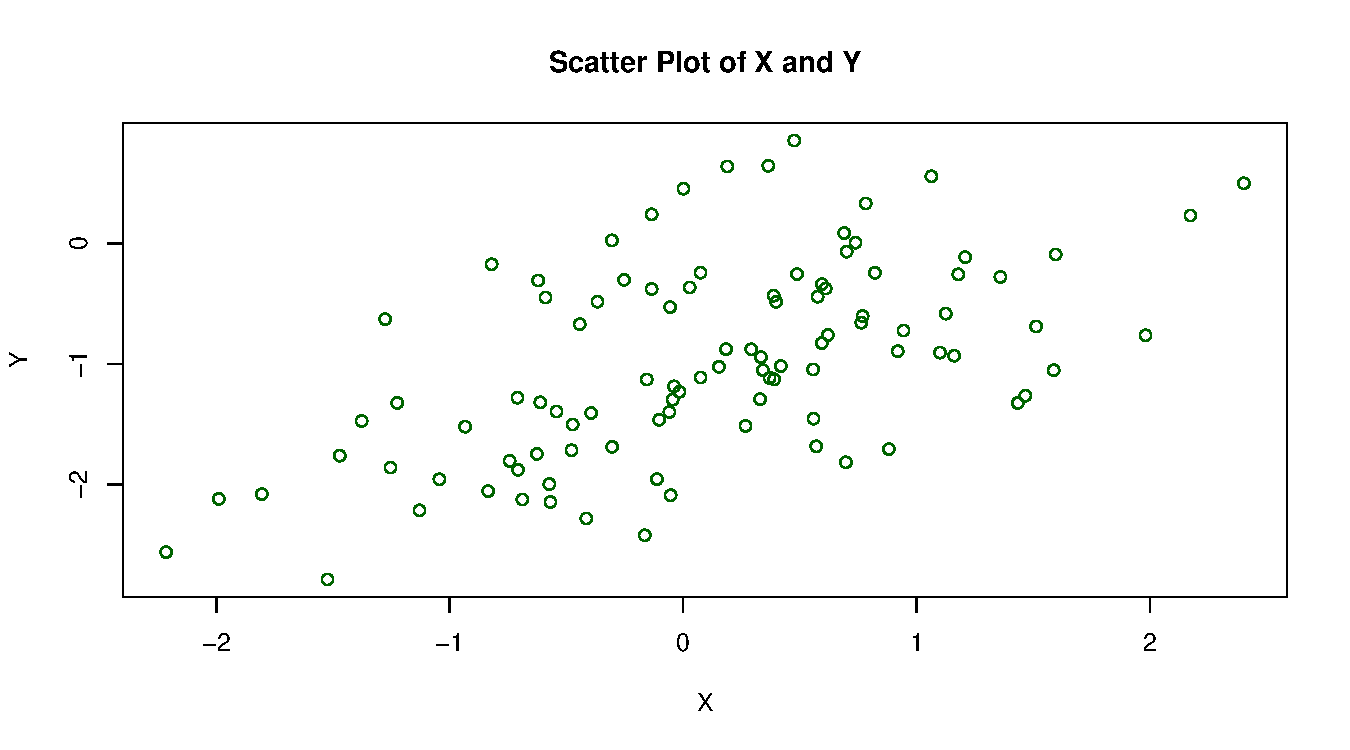
\includegraphics[width=0.9\linewidth]{Images/Prob2-Ex13-i-d.pdf}
\end{center}

The scatter plot shows that the \xr and \yr roughly has a linear correlation. The relationship is very noisy, and the noise is larger in scale compare to the previous 2 data sets.
\bigskip



(e)
The coefficients in the results are
\[
    \hat\beta_0 = -1.0263848,\qquad 
    \hat\beta_1 = 0.4992577
\]
That is, our linear model can be described as 
\[
    \yr \sim \hat\beta_0 + \hat\beta_1\xr 
    = -1.0263848 + 0.4992577\xr
\]
This model is very close to the original population model without noise $Y = -1 + 0.5X$.

Comparing with the original $\beta_0$ and $\beta_1$, we calculate in \code{R}
\[
    |\hat\beta_0 - \beta_0| = 0.02638483 \quad 
    |\hat\beta_1 - \beta_1| = 0.0007422703
\]
We can see that our estimated coefficients $\hat\beta_0$, $\hat\beta_1$ are close to the population values $\beta_0$ and $\beta_1$. The difference is caused by the random noise $\epsilon$. 
Also we can see that $\hat\beta_1$ is very close to $\beta_1$. This is expected, as our random noise $\epsilon$ is symmetrical, i.e. with mean 0.
\bigskip




(f)
\begin{center}
    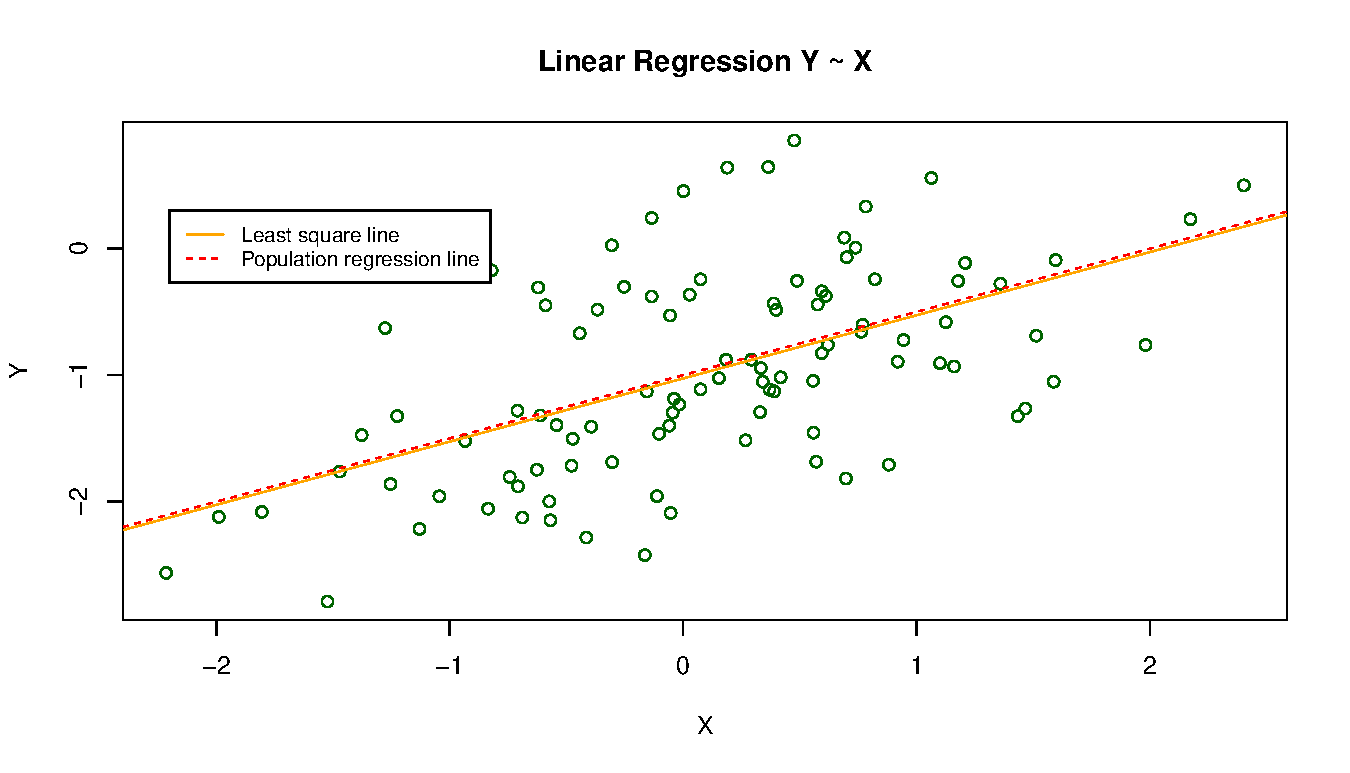
\includegraphics[width=0.9\linewidth]{Images/Prob2-Ex13-i-f.pdf}
    
    % Comments
    \parbox{0.65\textwidth}{\textit{In the plot, the \textcolor{myorange}{orange line} represents the least square line. The \textcolor{red}{red dotted line} represents the population regression line. The two lines are very close. Thus we chose dotted line for the population line to differentiate it from the other line.
    }}
\end{center}
\bigskip




(g)
Using commands in the \code{R} file \code{Prob2-Ex13-Part1.R}, we have the following result for the polynomial fitting 
\begin{verbatim}
(Intercept)           x      I(x^2) 
-0.96029949  0.51201261 -0.08324484
\end{verbatim}
or 
\[
    \yr \sim \hat{\beta}_0 + \hat{\beta}_1\xr + \hat{\beta}_2 \xr^2
    =
    -0.96029949
    + 0.51201261 \xr 
    -0.08324484 \xr^2 
\]

In order to compare the result with the linear regression, we calculate the residual sum of squares (RSS) for both cases.
\ba 
    \rss_{\tx{linear}} = 44.50945,\qquad 
    \rss_{\tx{quadratic}} = 43.62426
\ea 
From the \rss point of view, the quadratic fitting performs better than the linear fitting, but the difference is not significant. In this case, the improvement on RSS is better than the previous cases, because our data set is more noisy. This improvement on RSS does not really mean the quadratic model performs better. In fact, in this case, the quadratic fitting captures more noise than the underlying pattern. 
\bigskip\bigskip




\noindent\textcolor{blue}{\textbf{Confidence Intervals}}\bigskip 

\qnum{j}
Here we give the 95\% confidence intervals for the coefficients $\beta_0$ and $\beta_1$.

\begin{itemize}
    \item \textbf{Less Noise}
    \[
        I_{\beta_0} = [-1.0460321, -0.9690449],\quad 
        I_{\beta_1} = [0.4570318, 0.5425441]
    \]
    Interval lengths:
    \ba 
        |I_{\beta_0}| =& |-1.0460321 - (-0.9690449)| = 0.0769872,\\
        |I_{\beta_1}| =& |0.4570318- 0.5425441| = 0.0855123
    \ea 

    
    \item \textbf{Original Noise}
    \[
        I_{\beta_0} = [-1.1150804, -0.9226122],\quad 
        I_{\beta_1} = [0.3925794,  0.6063602]
    \]
    Interval lengths:
    \ba 
        |I_{\beta_0}| =& |-1.1150804 -( -0.9226122)| = 0.1924682,\\
        |I_{\beta_1}| =& |0.3925794-  0.6063602| = 0.2137808
    \ea 
    
    \item \textbf{More Noise}
    \[
        I_{\beta_0} = [-1.1611125, -0.8916571],\quad 
        I_{\beta_1} = [0.3496112, 0.6489043]
    \]
    Interval lengths:
    \ba 
        |I_{\beta_0}| =& |-1.1611125- (-0.8916571)| = 0.2694554,\\
        |I_{\beta_1}| =& |0.3496112- 0.6489043| = 0.2992931
    \ea 
\end{itemize}

Here, we compare the results by comparing the lengths of the confidence intervals. As we can see, the interval lengths increase as we go from less noise to more noise. This is consistent with the increase in the noise. When noise is heavier, our estimate would become less accurate, and thus result in larger confidence intervals.
\bigskip




























\bigskip\bigskip
\begin{center}
    \textcolor{myfirebrick}{\textbf{Exercise 14}}
\end{center}

\newcommand{\xar}{\textcolor{myfirebrick}{\code{x1}} }
\newcommand{\xbr}{\textcolor{myfirebrick}{\code{x2}} }

\qnum{a}
The linear model is 
\[
    Y = 2 + 2X_1 + 0.3X_2 + \epsilon 
\]
where $\epsilon\sim N(0, 0.1^2)$. The regression coefficients are corresponding to $X_0 = 1$, $X_1$ and $X_2$
\[
    \beta_0 = 2,\quad 
    \beta_1 = 2,\quad 
    \beta_2 = 0.3
\]


\qnum{b}
The correlation is 
\[
    \text{cor}(\xar, \xbr) = 0.8351212
\]

\begin{center}
    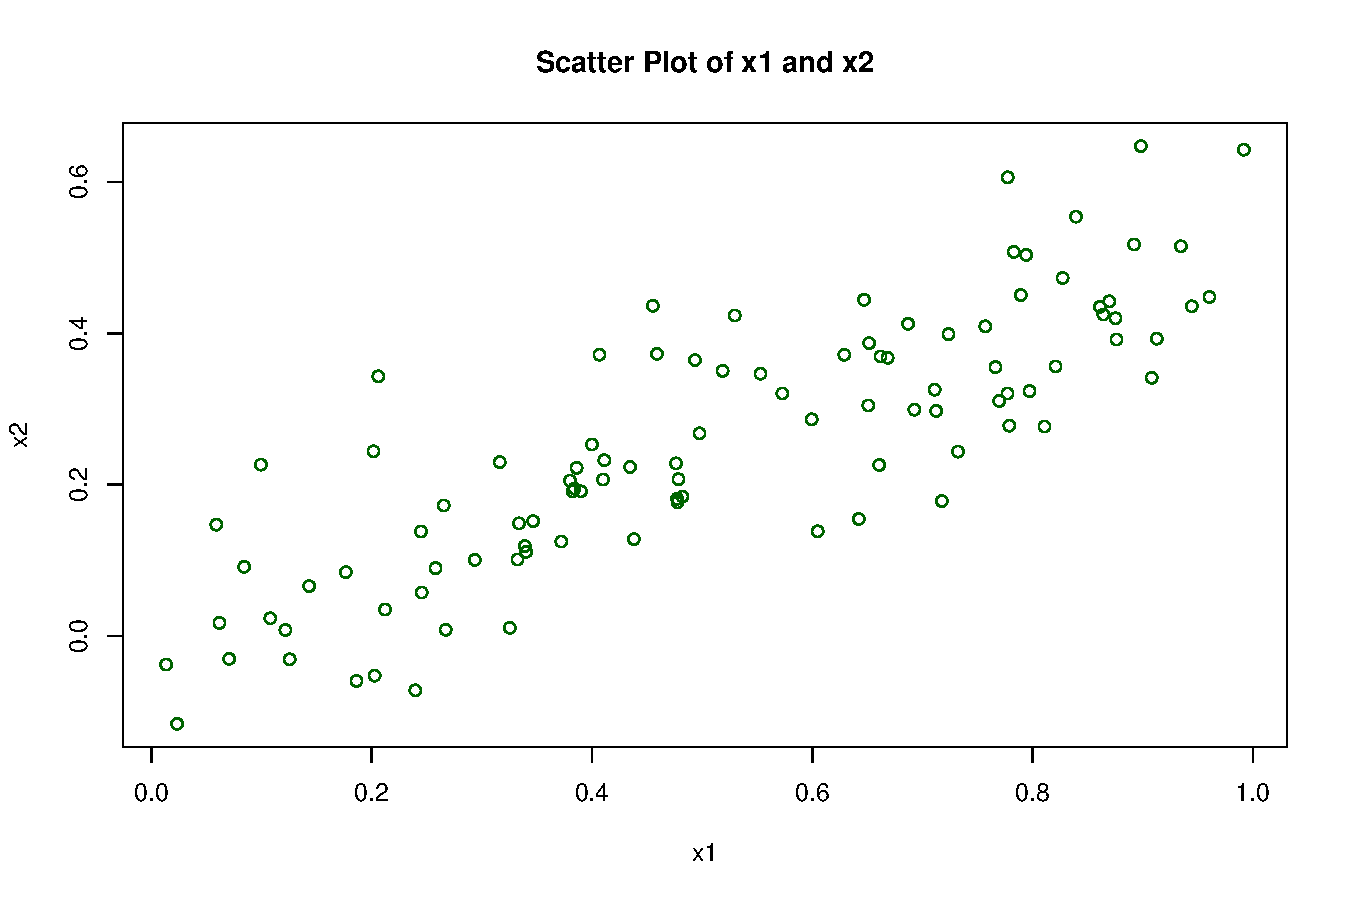
\includegraphics[width=0.9\linewidth]{Images/Prob2-Ex14-b.pdf}
\end{center}
\bigskip


\qnum{c}
Using linear regression, we have the least square regression coefficients as 
\[
    \hat\beta_0 = 2.130500,\quad 
    \hat\beta_1 = 1.439555,\quad 
    \hat\beta_2 = 1.009674
\]
The least squares regression model can be described as 
\[
    \yr \sim\hat\beta_0 + \hat\beta_1\xar + \hat\beta_2\xbr
    = 2.130500 + 
    1.439555\xar +
    1.009674\xbr 
\]

The differences between all estimated coefficients and true coefficients are calculated below.
\[
    |\beta_0 - \hat\beta_0| = 0.1304996,\quad 
    |\beta_1 - \hat\beta_1| = 0.5604446,\quad 
    |\beta_2 - \hat\beta_2| = 0.7096742
\]
From these numbers, we can see that $\beta_0$ is closest to the true value, while $\beta_1$ is quite faraway from the true value and $\beta_2$ is very faraway from the true value.

For the hypothesis tests:
\begin{itemize}
    \item $H_0: \beta_1 = 0$\\
    The $t$-value is 1.996 and this gives a $p$-value of 0.0487. If we use a significance level of 0.05, we would \textbf{reject} $H_0$ and accept the alternative hypothesis $H_1: \beta_1 \ne 0$, i.e. \yr is linearly correlated with \xar. 
    
    However, the $p$-value is close to the significance level 0.05. This means that using any significance level lower than 0.0487, e.g. 0.01, would result in acceptance of $H_0$ and the conclusion that \yr is not linearly correlated with \xar.
    
    \item $H_0: \beta_2 = 0$\\
    The $t$-value is 0.891 and this gives a $p$-value of 0.3754. If we use a significance level of 0.05, we would \textbf{not reject} $H_0$, i.e. \yr is not linearly correlated with \xbr.
\end{itemize}
\bigskip





\qnum{d}
Using linear regression, we have the least square regression coefficients as 
\[
    \hat\beta_0 = 2.112394 ,\quad 
    \hat\beta_1 = 1.975929 
\]
The least squares regression model can be described as 
\[
    \yr \sim\hat\beta_0 + \hat\beta_1\xar 
    = 2.112394 + 
    1.975929\xar 
\]

The differences between all estimated coefficients and true coefficients are calculated below.
\[
    |\beta_0 - \hat\beta_0| = 0.1123936,\quad 
    |\beta_1 - \hat\beta_1| = 0.0240710
\]
From these numbers, we can see that $\beta_0$ and $\beta_1$ are both close to the true value.
\bigskip

For the hypothesis test
\[
    H_0: \beta_1 = 0
\]
The $t$-value is 4.986 and this gives a $p$-value of $2.66\times 10^{-6}$. If we use a significance level of 0.05, or any common levels, we would \textbf{reject} $H_0$ and accept the alternative hypothesis $H_1: \beta_1 \ne 0$, i.e. \yr is linearly correlated with \xar. 
\bigskip
    
    

\qnum{e}
Using linear regression, we have the least square regression coefficients as 
\[
    \hat\beta_0 = 2.389949 ,\quad 
    \hat\beta_1 = 2.899585 
\]
The least squares regression model can be described as 
\[
    \yr \sim\hat\beta_0 + \hat\beta_1\xbr 
    = 2.389949 + 
    2.899585\xbr 
\]

The differences between all estimated coefficients and true coefficients are calculated below.
\[
    |\beta_0 - \hat\beta_0| = 0.3899491,\quad 
    |\beta_1 - \hat\beta_1| = 2.599585
\]
From these numbers, we can see that $\beta_0$ is not faraway from the true value but $\beta_1$ is very different from the true value.
\bigskip

For the hypothesis test
\[
    H_0: \beta_1 = 0
\]
The $t$-value is 4.58 and this gives a $p$-value of $1.37\times 10^{-5}$. If we use a significance level of 0.05, or any common levels, we would \textbf{reject} $H_0$ and accept the alternative hypothesis $H_1: \beta_1 \ne 0$, i.e. \yr is linearly correlated with \xbr.
\bigskip


\qnum{f}
The results obtained in (c)-(e) do not contradict each other. The reason that we conclude that \xbr is not significantly correlated with \yr in the multivariate linear regression tests and that \xbr is correlated with \yr with statistical significance in the univariate linear regression tests is that, \xar and \xbr, or equivalently $X_1$ and $X_2$, are very correlated.
\bigskip 



\qnum{g}

\begin{center}
    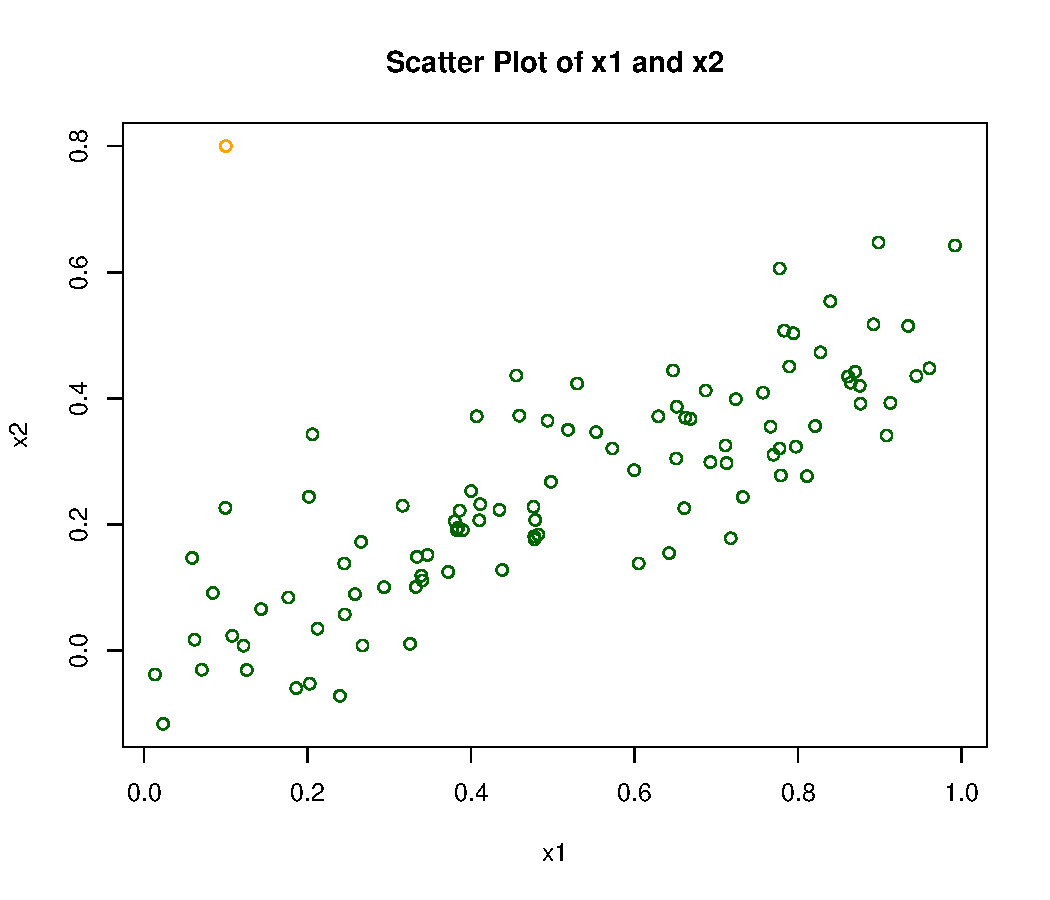
\includegraphics[width=0.7\linewidth]{Images/Prob2-Ex14-g-scatter.pdf}
    
    
    % Comments
    \parbox{0.65\textwidth}{\textit{In the plot, the \textcolor{myorange}{orange dot} represents the added data point.
    }}
\end{center}
\bigskip\bigskip

(c)
Using linear regression, we have the least square regression coefficients as 
\[
    \hat\beta_0 = 2.2266917,\quad 
    \hat\beta_1 = 0.5394397,\quad 
    \hat\beta_2 = 2.5145694
\]
The least squares regression model can be described as 
\[
    \yr \sim\hat\beta_0 + \hat\beta_1\xar + \hat\beta_2\xbr
    = 2.2266917 + 
    0.5394397\xar +
    2.5145694\xbr 
\]

The differences between all estimated coefficients and true coefficients are calculated below.
\[
    |\beta_0 - \hat\beta_0| = 0.2266917,\quad 
    |\beta_1 - \hat\beta_1| = 1.4605603,\quad 
    |\beta_2 - \hat\beta_2| = 2.2145694
\]
From these numbers, we can see that $\beta_0$ is closest to the true value, while $\beta_1$ and $\beta_2$ are both very faraway from the true value.

For the hypothesis tests:
\begin{itemize}
    \item $H_0: \beta_1 = 0$\\
    The $p$-value is 0.36458. If we use a significance level of 0.05, we would \textbf{not reject} $H_0$, i.e. \yr is not linearly correlated with \xar. 
    
    \item $H_0: \beta_2 = 0$\\
    The $p$-value is 0.00614. If we use a significance level of 0.05 or 0.01, we would \textbf{reject} $H_0$, i.e. \yr is linearly correlated with \xbr.
\end{itemize}
\bigskip





(d)
Using linear regression, we have the least square regression coefficients as 
\[
    \hat\beta_0 = 2.256927 ,\quad 
    \hat\beta_1 = 1.765695 
\]
The least squares regression model can be described as 
\[
    \yr \sim\hat\beta_0 + \hat\beta_1\xar 
    = 2.256927 + 
    1.765695\xar 
\]

The differences between all estimated coefficients and true coefficients are calculated below.
\[
    |\beta_0 - \hat\beta_0| = 0.2569274,\quad 
    |\beta_1 - \hat\beta_1| = 0.2343045
\]
From these numbers, we can see that $\beta_0$ and $\beta_1$ are both close to the true value.
\bigskip

For the hypothesis test
\[
    H_0: \beta_1 = 0
\]
The $p$-value is $4.29\times 10^{-5}$. If we use a significance level of 0.05, or any common levels, we would \textbf{reject} $H_0$ and accept the alternative hypothesis $H_1: \beta_1 \ne 0$, i.e. \yr is linearly correlated with \xar. 
\bigskip
    
    

(e)
Using linear regression, we have the least square regression coefficients as 
\[
    \hat\beta_0 = 2.345107 ,\quad 
    \hat\beta_1 = 3.119050 
\]
The least squares regression model can be described as 
\[
    \yr \sim\hat\beta_0 + \hat\beta_1\xbr 
    = 2.345107 + 
    3.119050\xbr 
\]

The differences between all estimated coefficients and true coefficients are calculated below.
\[
    |\beta_0 - \hat\beta_0| = 0.3451069,\quad 
    |\beta_1 - \hat\beta_1| = 2.8190497
\]
From these numbers, we can see that $\beta_0$ is not faraway from the true value but $\beta_1$ is very different from the true value.
\bigskip

For the hypothesis test
\[
    H_0: \beta_1 = 0
\]
The $p$-value is $1.25\times 10^{-6}$. If we use a significance level of 0.05, or any common levels, we would \textbf{reject} $H_0$ and accept the alternative hypothesis $H_1: \beta_1 \ne 0$, i.e. \yr is linearly correlated with \xbr.
\bigskip\bigskip


\noindent\textcolor{blue}{\textbf{Summary}}\bigskip

Adding the data point completely changed $\hat\beta_1$ and $\hat\beta_2$ and resulted in different hypothesis tests on them, i.e. accepting that $\xbr$ is linearly correlated with $\yr$ but not $\xar$.
The change is not large however in the (d) and (e) models. The estimates and hypothesis tests gave similar results in both cases.
\bigskip\bigskip






\begin{center}
    \textcolor{myfirebrick}{\textbf{Exercise 15}}
\end{center}

\qnum{a}
Using \code{R}, we calculated all the least square regression coefficients.

\begin{verbatim}
           beta_0       beta_1
crim     24.03311  -0.41519028
zn       20.91758   0.14213999
indus    29.75490  -0.64849005
chas     22.09384   6.34615711
nox      41.34587 -33.91605501
rm      -34.67062   9.10210898
age      30.97868  -0.12316272
dis      18.39009   1.09161302
rad      26.38213  -0.40309540
tax      32.97065  -0.02556810
ptratio  62.34463  -2.15717530
black    10.55103   0.03359306
lstat    34.55384  -0.95004935
\end{verbatim}

The following plots are scatter plots for each pair of the predictor and the response variable. The orange line represents the least square regression line.

\begin{center}
    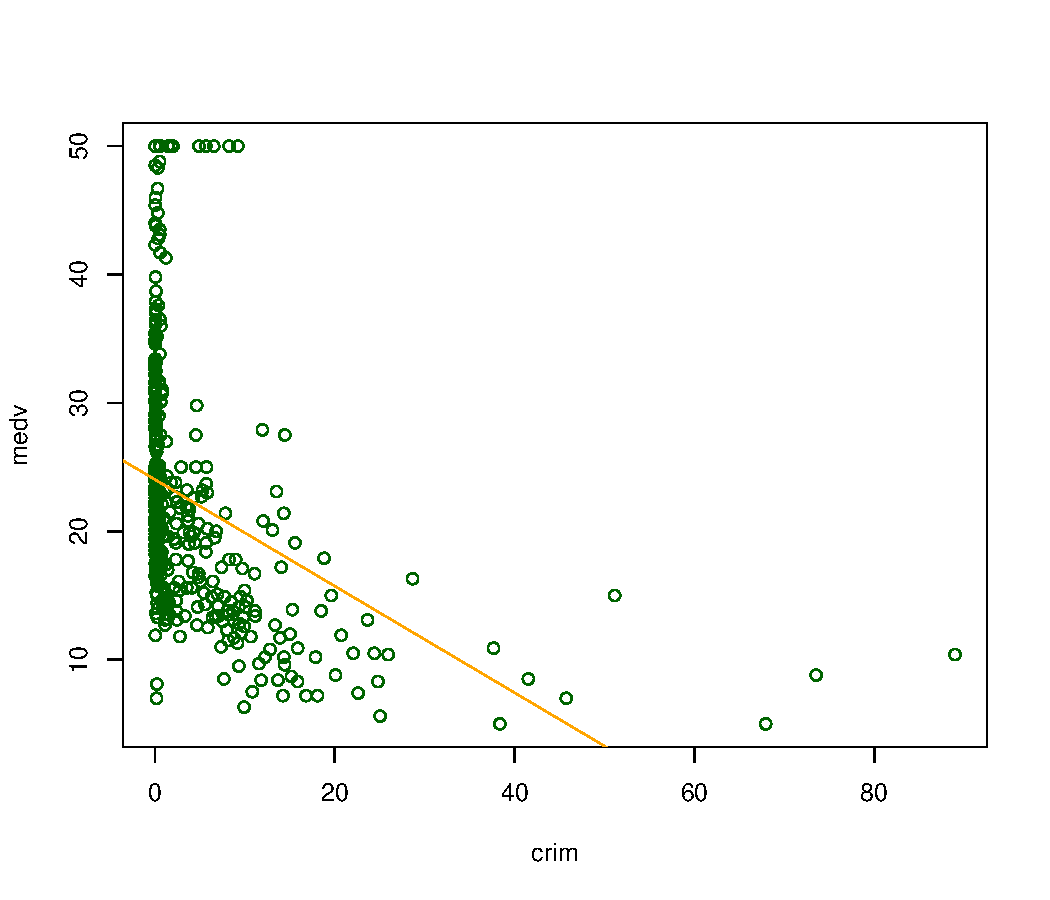
\includegraphics[width=0.45\linewidth]{Images/Prob2-Ex15-a-1.pdf}
    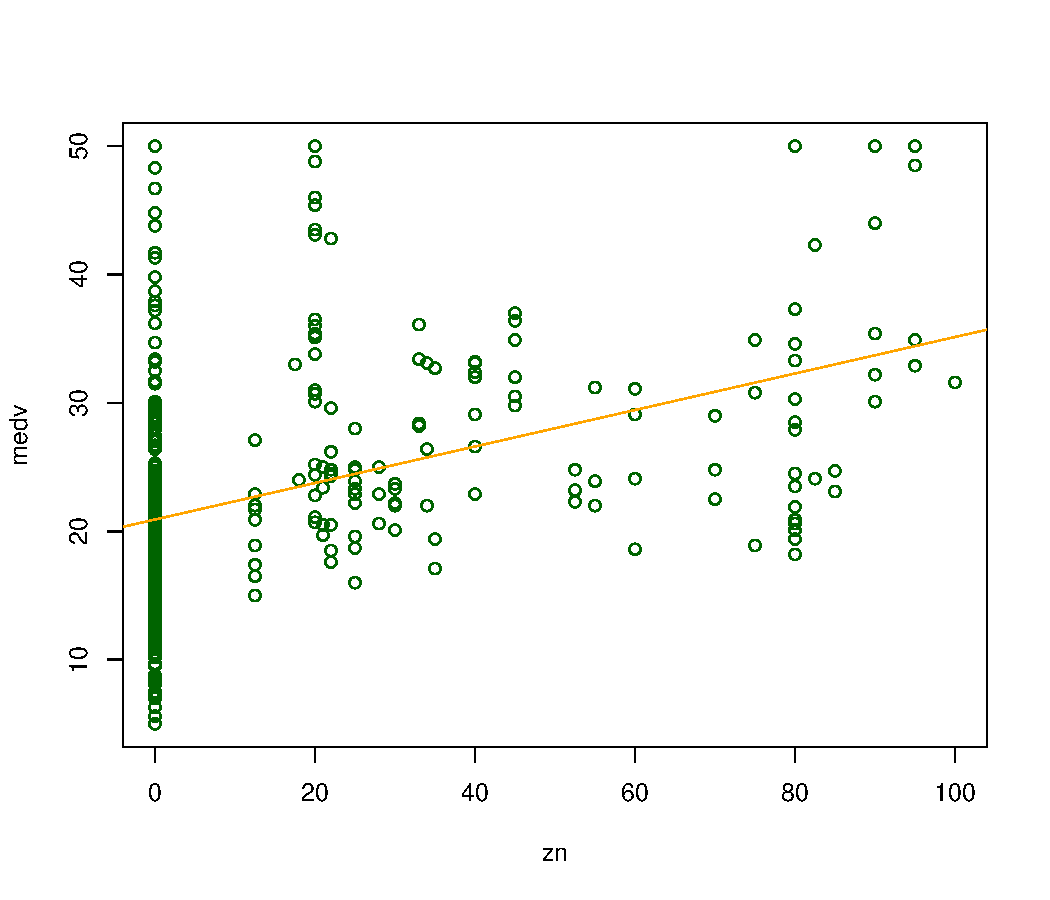
\includegraphics[width=0.45\linewidth]{Images/Prob2-Ex15-a-2.pdf}
    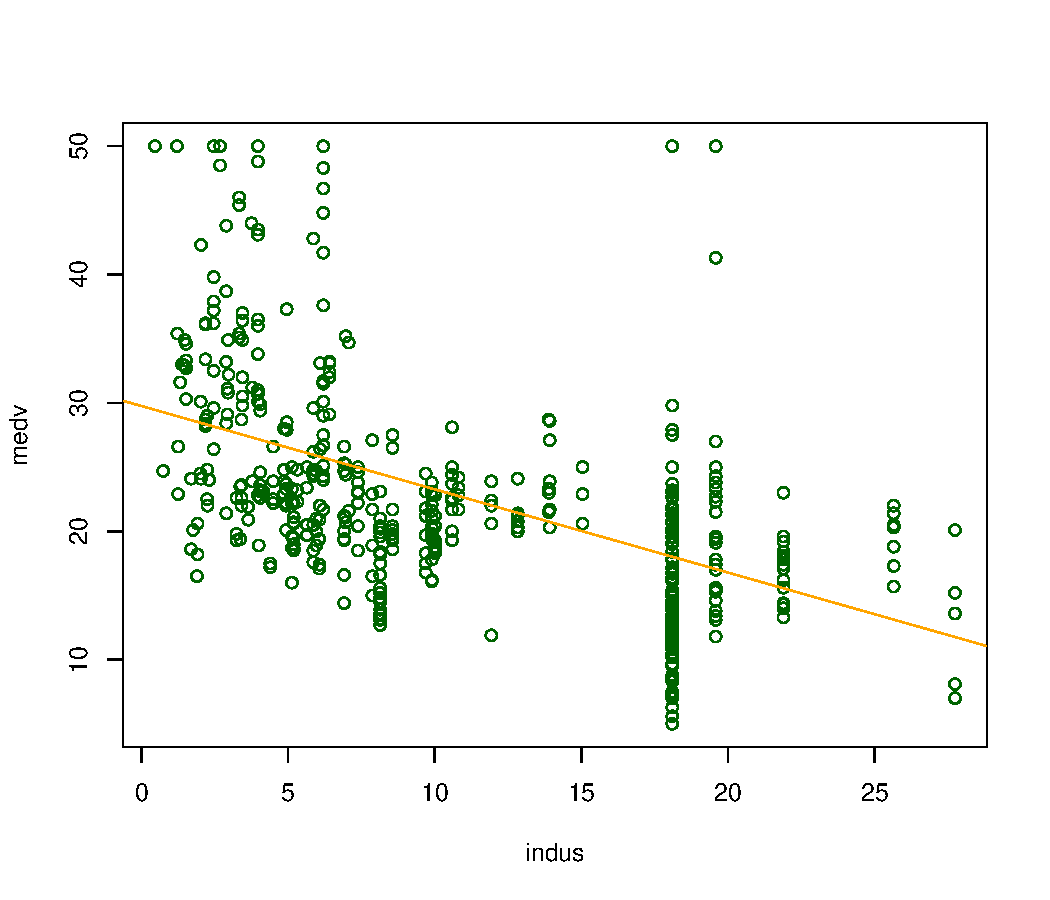
\includegraphics[width=0.45\linewidth]{Images/Prob2-Ex15-a-3.pdf}
    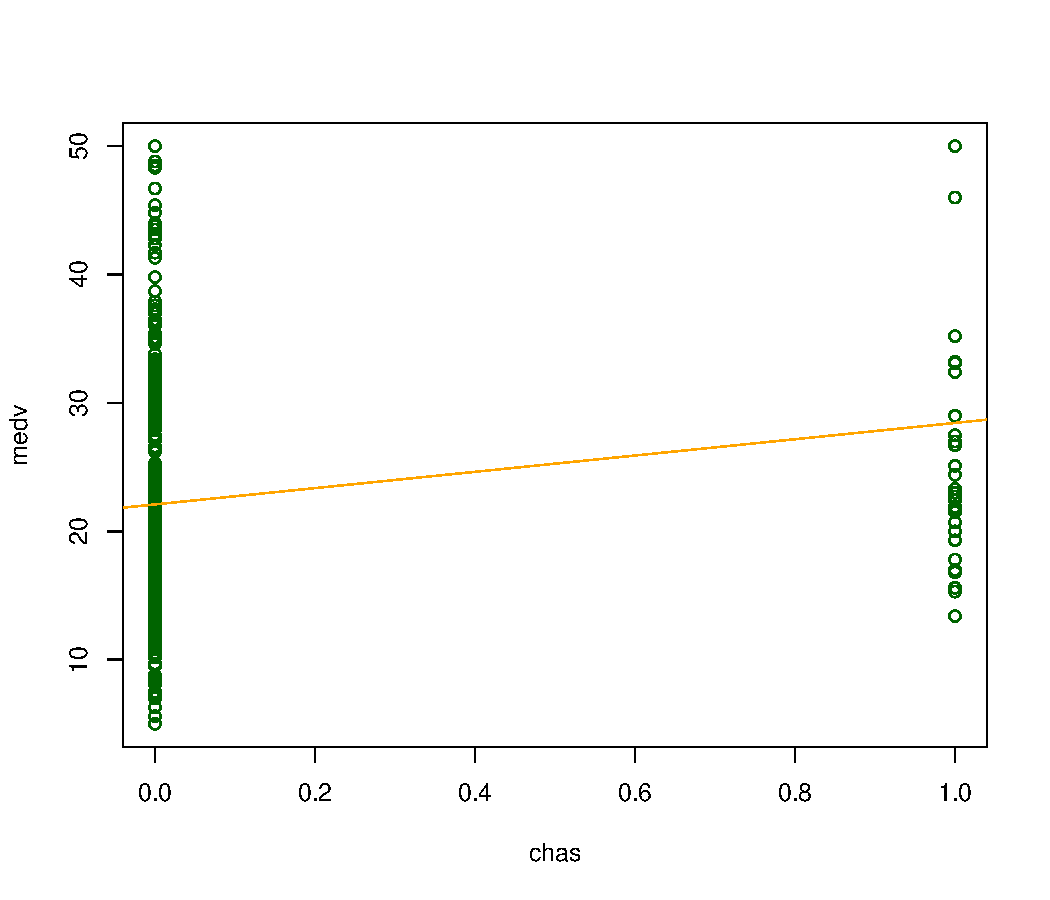
\includegraphics[width=0.45\linewidth]{Images/Prob2-Ex15-a-4.pdf}
    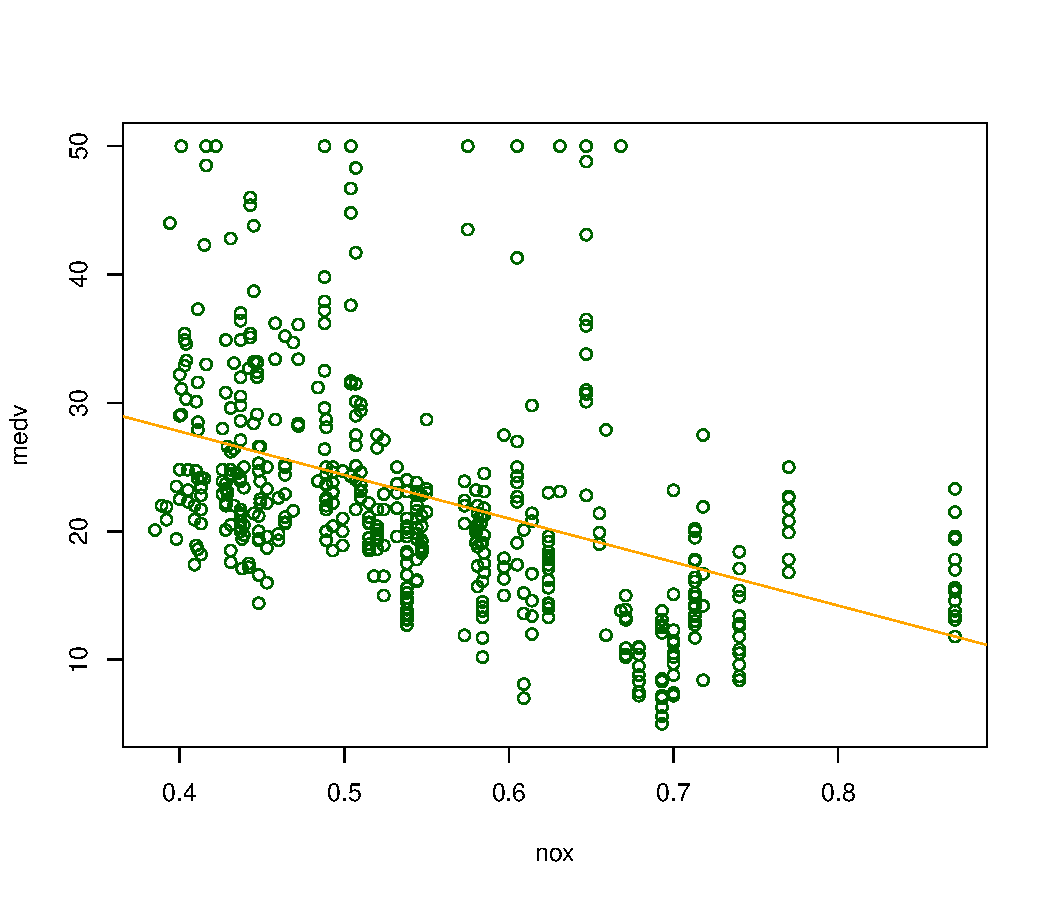
\includegraphics[width=0.45\linewidth]{Images/Prob2-Ex15-a-5.pdf}
    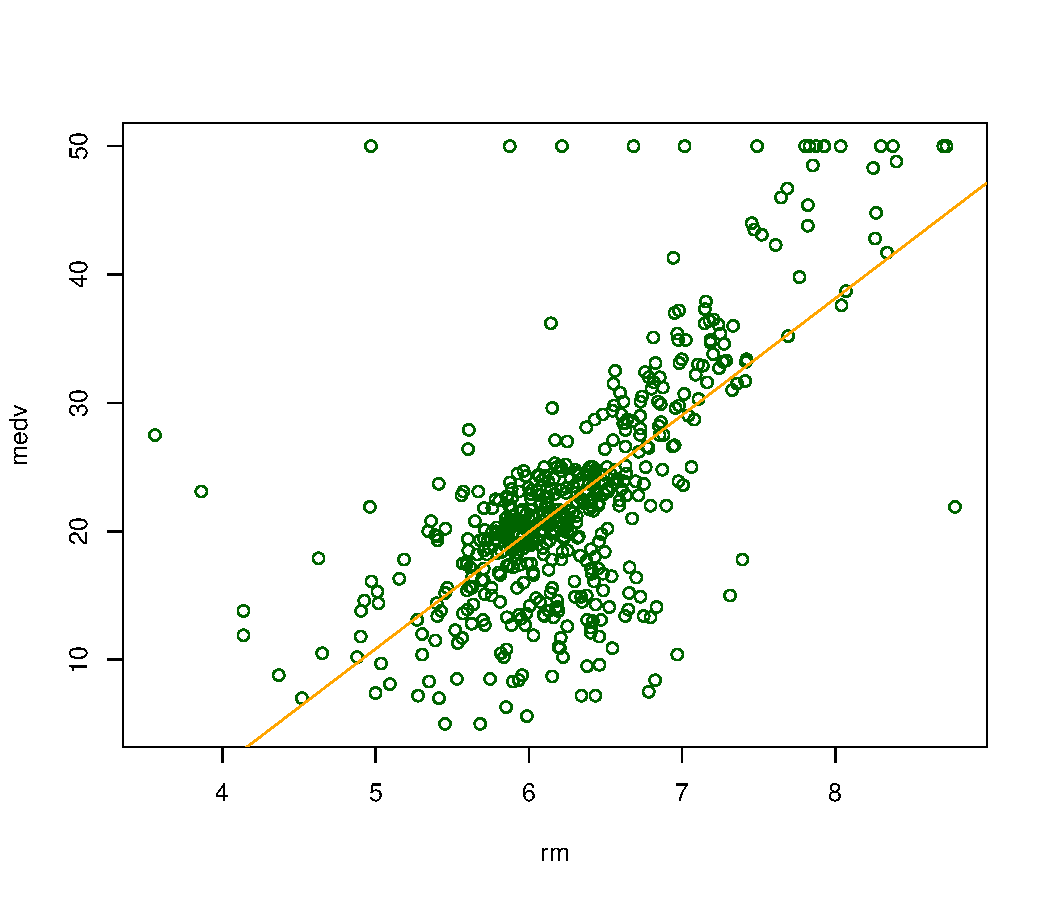
\includegraphics[width=0.45\linewidth]{Images/Prob2-Ex15-a-6.pdf}
    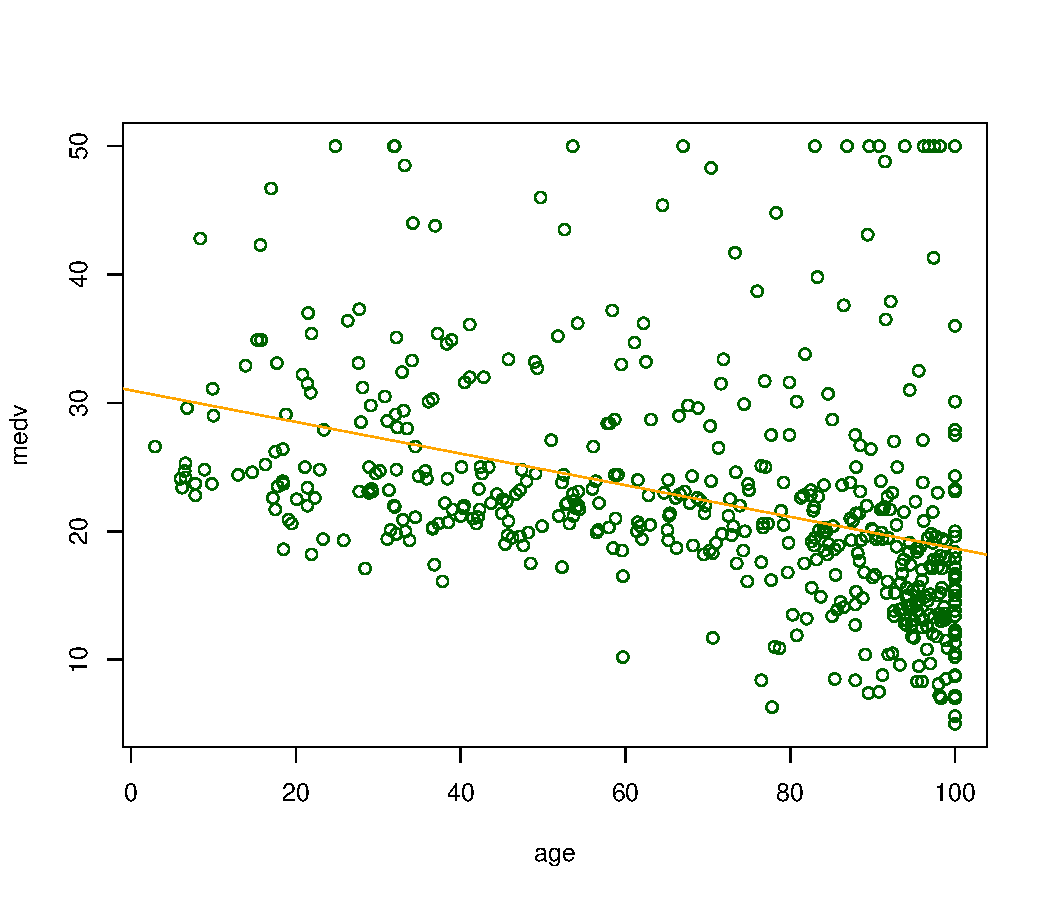
\includegraphics[width=0.45\linewidth]{Images/Prob2-Ex15-a-7.pdf}
    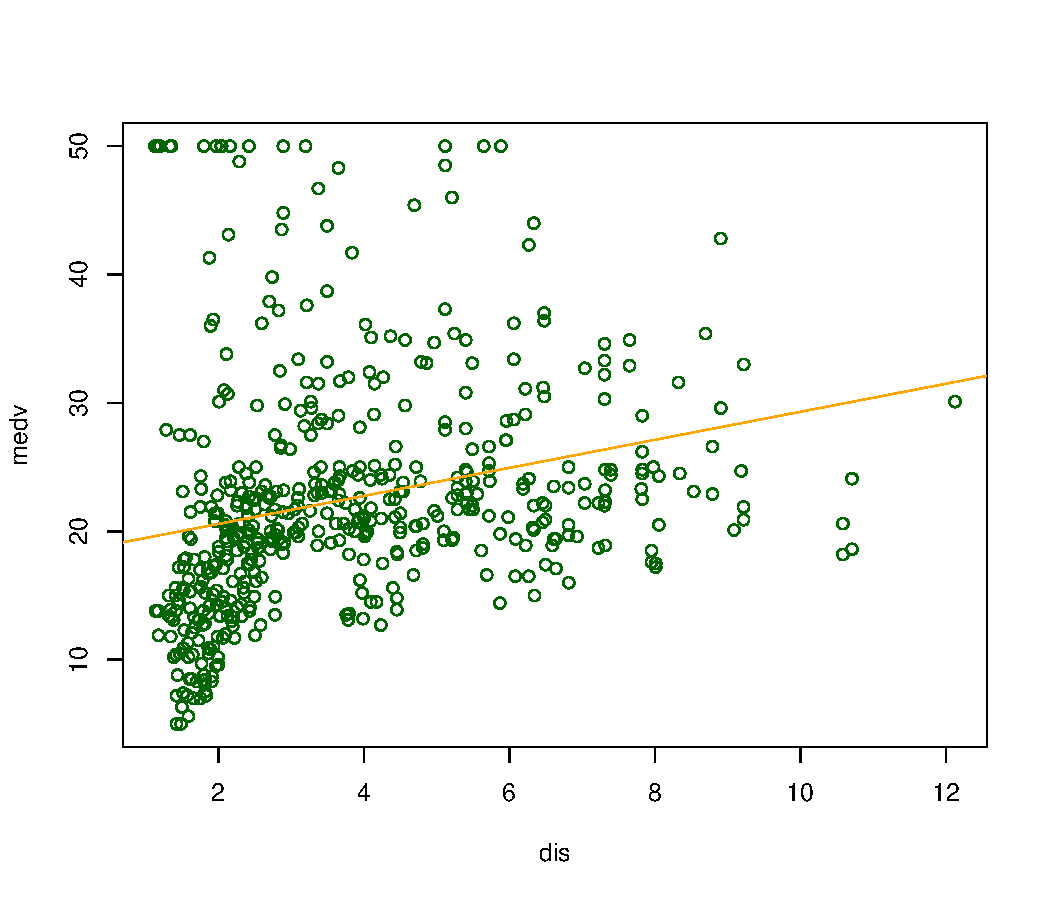
\includegraphics[width=0.45\linewidth]{Images/Prob2-Ex15-a-8.pdf}
    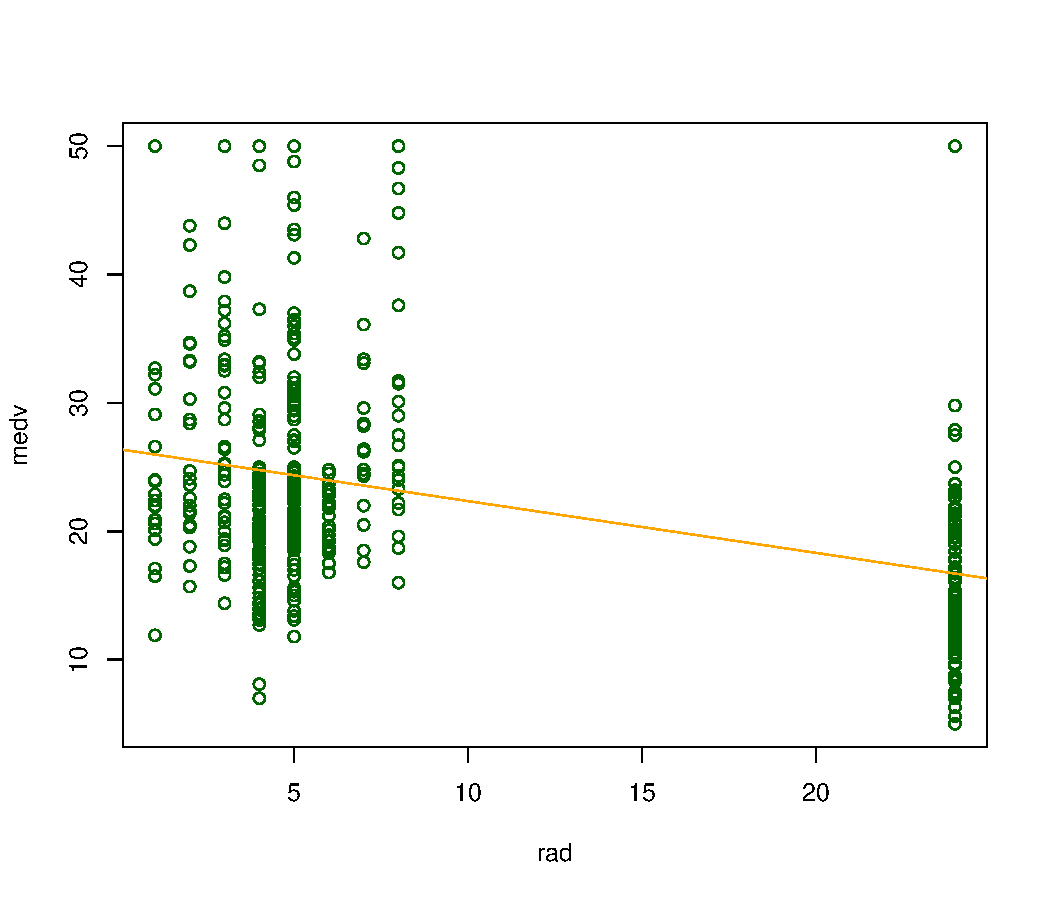
\includegraphics[width=0.45\linewidth]{Images/Prob2-Ex15-a-9.pdf}
    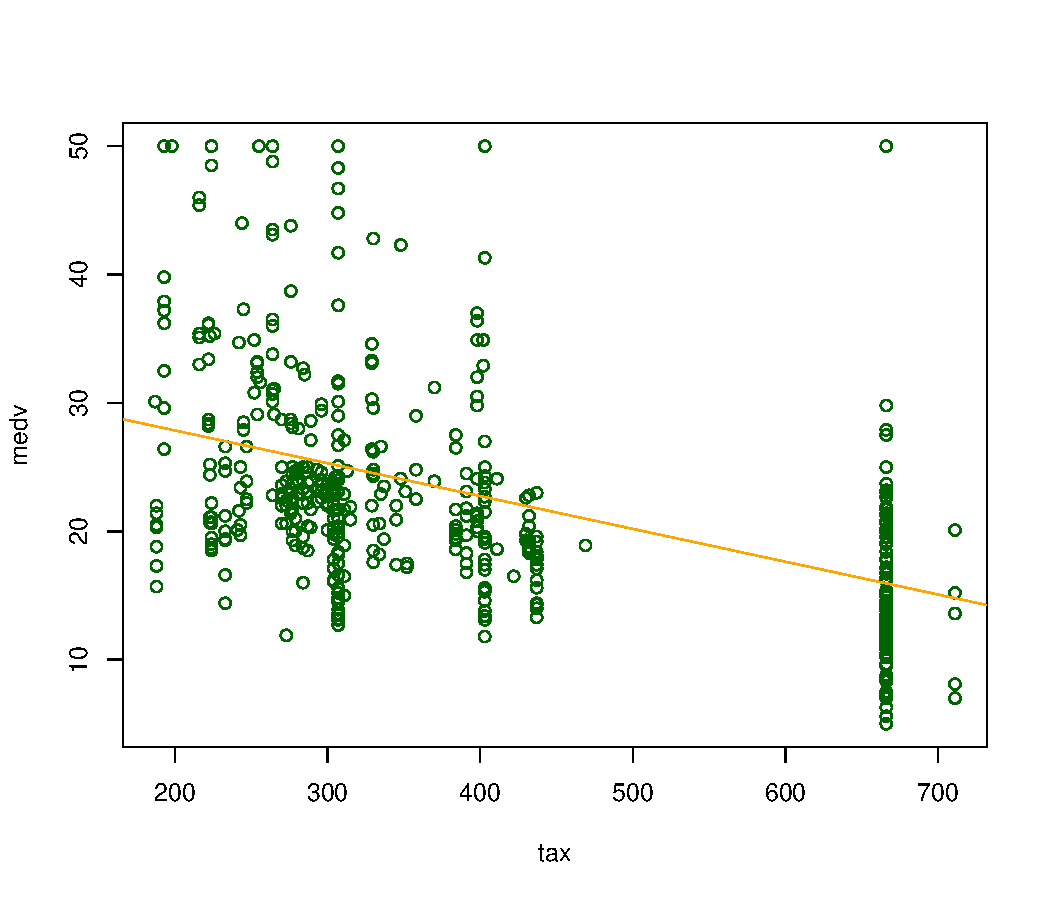
\includegraphics[width=0.45\linewidth]{Images/Prob2-Ex15-a-10.pdf}
    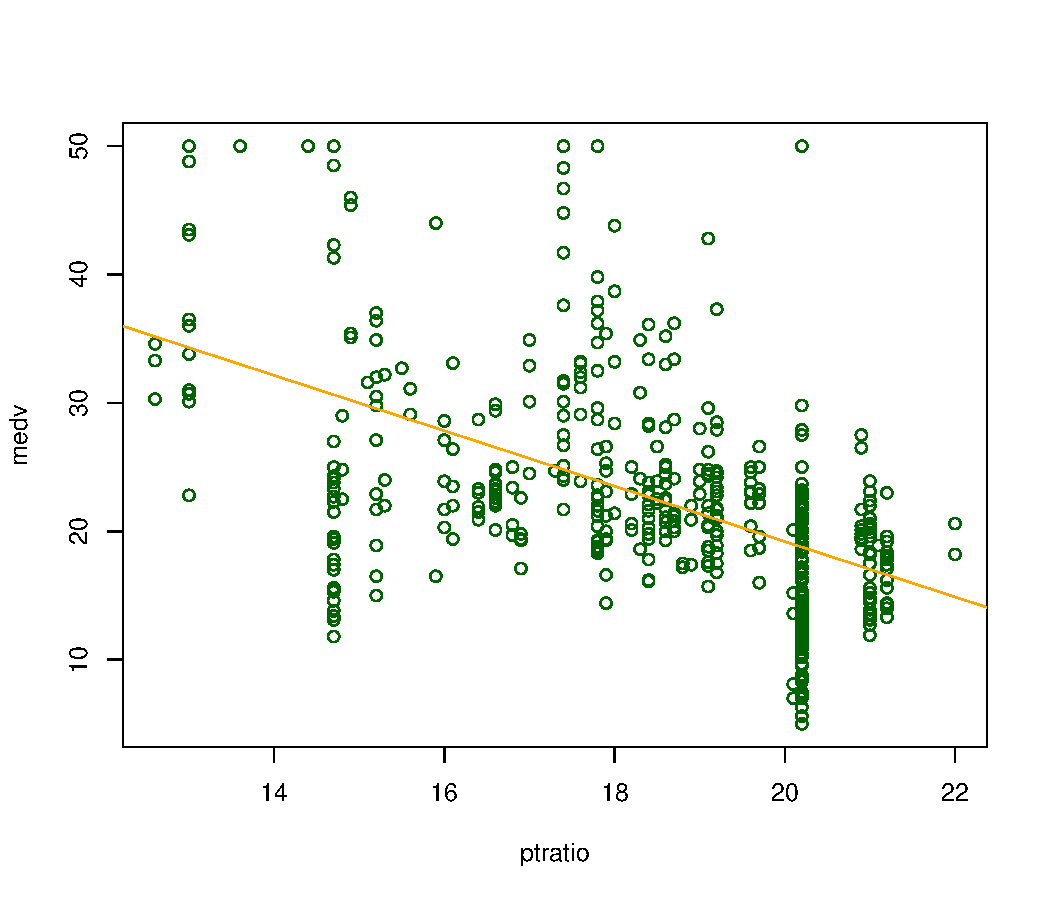
\includegraphics[width=0.45\linewidth]{Images/Prob2-Ex15-a-11.pdf}
    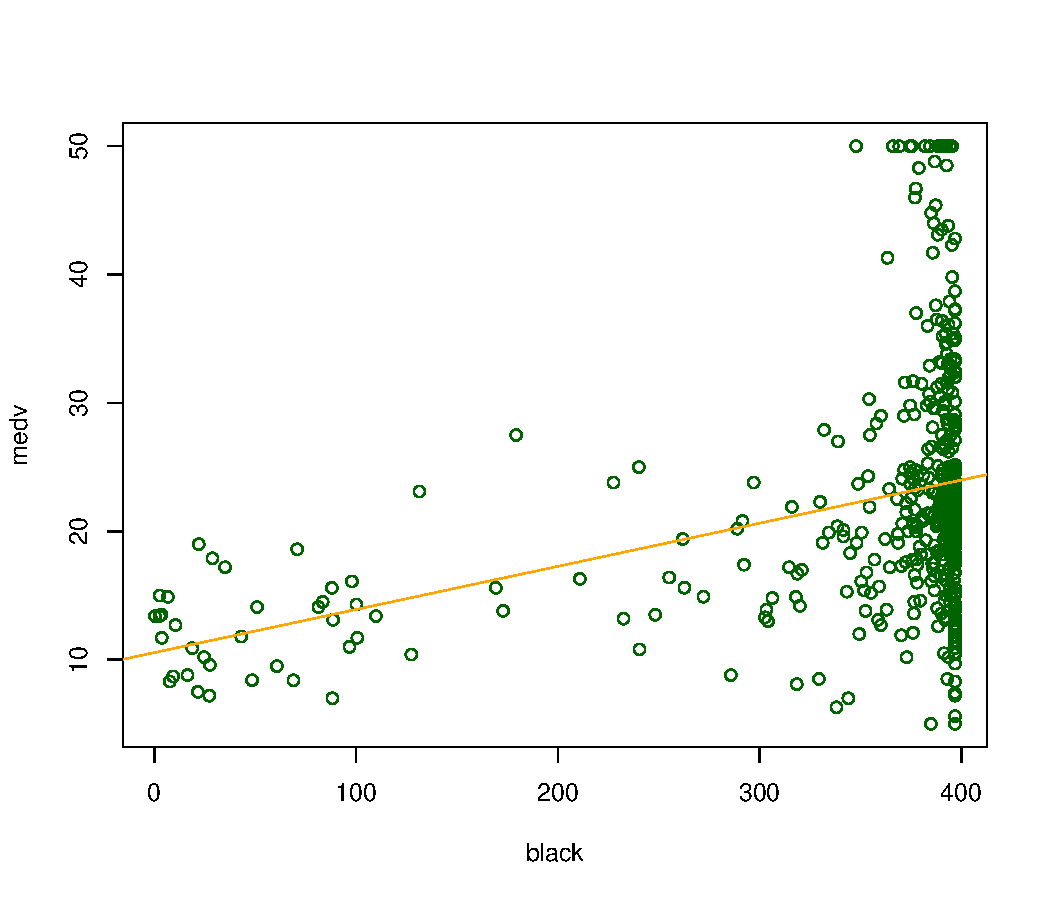
\includegraphics[width=0.45\linewidth]{Images/Prob2-Ex15-a-12.pdf}
    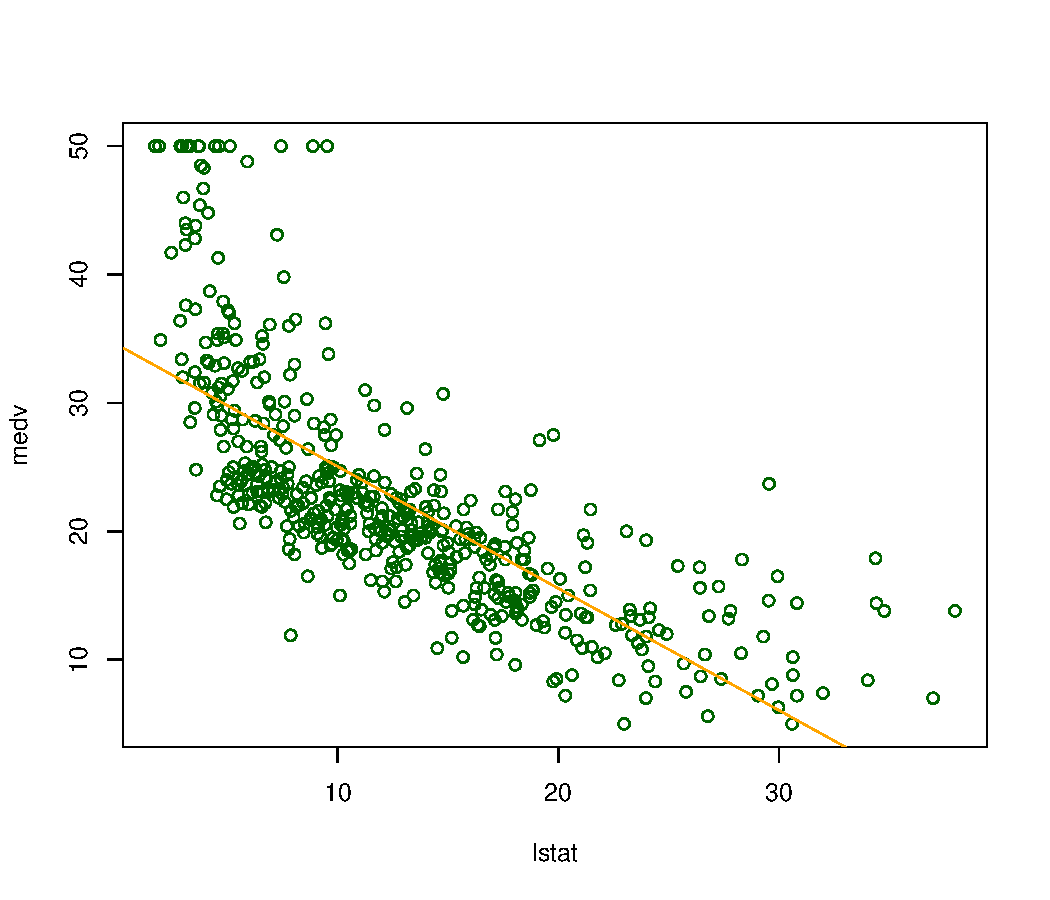
\includegraphics[width=0.45\linewidth]{Images/Prob2-Ex15-a-13.pdf}
\end{center}

From the graph, we can see that \code{nox}, \code{rm}, \code{age}, \code{dis}, \code{ptratio} and \code{lstat} seem to have statistically significant association with the response.
\bigskip

We also give the $p$-values below.
\begin{verbatim}
               beta_0       beta_1
crim    1.341723e-227 1.173987e-19
zn      9.489803e-195 5.713584e-17
indus   6.704987e-173 4.900260e-31
chas    7.002789e-208 7.390623e-05
nox      9.866245e-80 7.065042e-24
rm       6.950229e-34 2.487229e-74
age     6.814198e-119 1.569982e-18
dis      4.008955e-78 1.206612e-08
rad     3.282092e-186 5.465933e-19
tax     5.519383e-136 5.637734e-29
ptratio  9.077444e-69 1.609509e-34
black    3.491585e-11 1.318113e-14
lstat   3.743081e-236 5.081103e-88
\end{verbatim}

From the $p$-values, we conclude that they all have statistically significant association with the response value.
\bigskip

Here, the $p$-values are very small. This might be the effect of large number of data points, which causes the $t$-distribution to have small tails. We should consider using lower significance levels or try other statistical methods to determine association.
\bigskip

\qnum{b}

Using \code{R}, we have the following result for the coefficients
\begin{verbatim}
Coefficients:
              Estimate Std. Error t value Pr(>|t|)    
(Intercept)  3.646e+01  5.103e+00   7.144 3.28e-12
crim        -1.080e-01  3.286e-02  -3.287 0.001087
zn           4.642e-02  1.373e-02   3.382 0.000778
indus        2.056e-02  6.150e-02   0.334 0.738288    
chas         2.687e+00  8.616e-01   3.118 0.001925
nox         -1.777e+01  3.820e+00  -4.651 4.25e-06
rm           3.810e+00  4.179e-01   9.116  < 2e-16
age          6.922e-04  1.321e-02   0.052 0.958229    
dis         -1.476e+00  1.995e-01  -7.398 6.01e-13
rad          3.060e-01  6.635e-02   4.613 5.07e-06
tax         -1.233e-02  3.760e-03  -3.280 0.001112
ptratio     -9.527e-01  1.308e-01  -7.283 1.31e-12
black        9.312e-03  2.686e-03   3.467 0.000573
lstat       -5.248e-01  5.072e-02 -10.347  < 2e-16
\end{verbatim}

That is, the coefficients are 
\[
    \beta = 
    \begin{pmatrix}
        36.45949\\ -0.1080114\\ 0.04642046\\ 0.02055863\\ 2.686734\\ -17.76661\\ 3.809865\\ 0.0006922246\\ -1.475567\\ 0.3060495\\ -0.01233459\\ -0.9527472\\ 0.009311683\\ -0.5247584
    \end{pmatrix}
\]

We use significance level of $0.05$. Then the following predictors have $p$-values less than the significance level 0.05:
\begin{center}
    \code{Intercept}, 
    \code{crim},
    \code{zn},
    \code{chas},
    \code{nox},
    \code{rm},
    \code{dis},
    \code{rad},
    \code{tax},
    \code{ptratio},
    \code{black},
    \code{lstat}
\end{center}
That is, all the predictors except \code{indus} and \code{age}.
For these predictors, we reject the null hypothesis $H_0$.
\bigskip




\qnum{c}
\begin{center}
    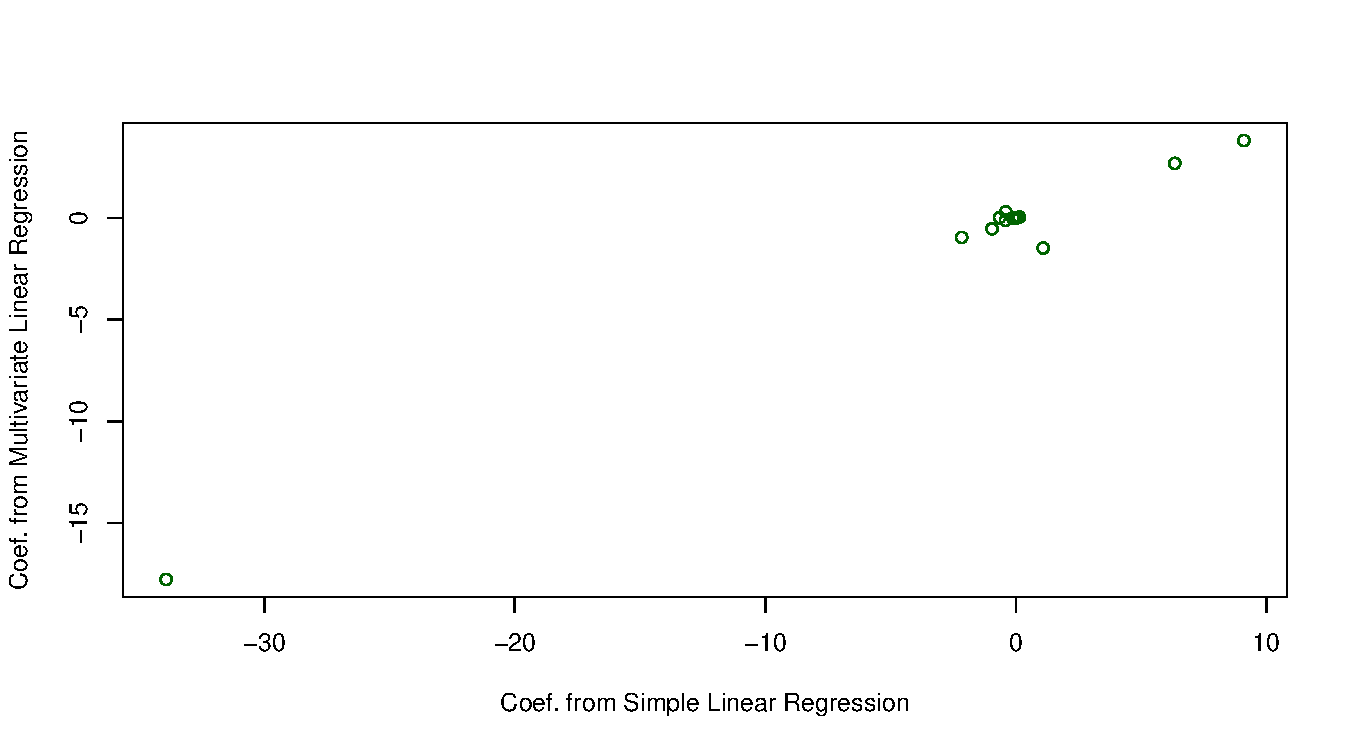
\includegraphics[width=1\linewidth]{Images/Prob2-Ex15-c.pdf}
\end{center}

Compared to (a), we have more predictors statistically associated to the response in (b).
\bigskip







\qnum{d}
Coefficients:
\begin{verbatim}
            beta_0        beta_1        beta_2        beta_3
crim     25.190479   -1.13640072  2.378483e-02 -1.488721e-04
zn       20.448597    0.64336518 -1.676457e-02  1.257022e-04
indus    37.080160   -2.80699408  1.404617e-01 -2.398890e-03
chas     22.093843    6.34615711            NA            NA
nox     -22.486390  315.09596351 -6.158267e+02  3.501860e+02
rm      241.310814 -109.39060642  1.649102e+01 -7.403937e-01
age      28.931102   -0.12241882  2.354563e-03 -2.317915e-05
dis       7.037894    8.59284424 -1.249528e+00  5.601936e-02
rad      30.251303   -3.79945390  6.163466e-01 -2.008638e-02
tax      52.216023   -0.16346964  3.029307e-04 -2.078684e-07
ptratio 312.286417  -48.69113602  2.839951e+00 -5.686478e-02
black    12.598120   -0.01703275  2.036076e-04 -2.224273e-07
lstat    48.649625   -3.86559278  1.487385e-01 -2.003868e-03
\end{verbatim}

$p$-values:
\begin{verbatim}
               beta_0       beta_1        beta_2       beta_3
crim    3.638793e-224 2.235435e-14  5.184482e-04 2.541096e-02
zn      1.301845e-185 1.055518e-08  1.941865e-05 7.981118e-05
indus    4.912614e-77 5.713973e-08  7.807276e-04 1.802575e-02
chas    7.002789e-208 7.390623e-05 7.002789e-208 7.390623e-05
nox      5.596479e-01 1.069282e-01  5.522193e-02 4.100152e-02
rm       4.853140e-07 2.505427e-06  8.952478e-06 1.461903e-04
age      2.160623e-20 5.435765e-01  5.493772e-01 3.096903e-01
dis      1.598664e-02 3.767574e-05  2.569178e-03 2.146307e-02
rad      1.871399e-28 3.814616e-03  9.907537e-04 4.819196e-04
tax      2.062352e-04 1.496461e-01  2.920043e-01 3.530609e-01
ptratio  4.108411e-02 7.071842e-02  7.001702e-02 5.900888e-02
black    7.700903e-07 7.819282e-01  5.323182e-01 6.408515e-01
lstat   6.294703e-132 2.329688e-28  9.177622e-12 7.428441e-07
\end{verbatim}

$p$-values from $F$-tests:
\begin{verbatim}
crim     1.448648e-26
zn       1.655884e-19
indus    4.415394e-35
chas     7.390623e-05
nox      2.561169e-23
rm       2.141469e-89
age      1.962401e-18
dis      4.735610e-12
rad      4.866503e-21
tax      9.824004e-28
ptratio  1.354349e-33
black    4.462765e-13
lstat   1.784655e-116
\end{verbatim}

From the $p$-values, we can see strong evidence that non-linear association exists.










 %%%%%%%%%%%%%%%%%%%%%%%%%%%%%%%%%%%%%%%%%%%%%%%%%%%%%

%     PROBLEM 3

 %%%%%%%%%%%%%%%%%%%%%%%%%%%%%%%%%%%%%%%%%%%%%%%%%%%%%

\newpage
\section*{Problem 3 [65 points]} 

Implement gradient descent algorithm for logistic regression and answer the following questions. In this question, you are asked to use your gradient descent implementation to train logistic regression models over Auto data set.
\subsubsection*{Initialization of the parameters} 

\begin{itemize}
\item Add $x_0 =1$ to data (all ones variable)
\item Set the learning rate $\alpha$ to 0.01 and iteration number to 1000. You may need to use different $\alpha$ and iteration number values if you observe they are not sufficient.
\item Initialize $\theta$'s as $0$'s -- $(\theta_0,\ldots, \theta_n) = (0,\ldots,0)$
\end{itemize}

\subsubsection*{Data Preprocessing} 

\begin{itemize}
\item  Create a binary variable, \quotes{mpg01}, that contains a 1 if mpg contains a value above its median, and a 0 if mpg contains a value below its median
\item Create a new data set called new.Auto by extracting the features mpg01, cylinders, displacement, horsepower, weight from Auto data set. Keep the order of the features as shown here in the new.Auto data set
\item Do feature scaling (mean normalization) over the input variables of the new.Auto data set to make gradient descent converge faster.
\item Use the new.Auto data set to answer the following questions
\end{itemize}

\subsection*{Logistic Regression } 

\begin{enumerate}
 \item[\textbf{3.1}] Implement the sigmoid function and make a plot of it by testing different inputs. $\big( g(z) = \frac{1}{1+e^{-z}}\big)$ [5 pt]
  \item[\textbf{3.2}] Perform logistic regression on the new.Auto data set in order to predict \quotes{mpg01} using the input variables: cylinders, displacement, horsepower, weight.  Report the parameters ($\theta$'s). [30 pt]
  \item[\textbf{3.3}] What is the error of the model over new.Auto data set? [10 pt]
  \item[\textbf{3.4}]   Use the model obtained in Q.3.1 to make predictions. What is the \quotes{mpg01} value for $(x_1,\ldots,x_4) =  (8,340,200,3500)$ (first, scale the data point with the parameters obtained earlier while normalizing the features) [5 pt]
\item[\textbf{3.5}]In this question, you are asked to test different learning rates. Run your gradient descent for 100 iterations at the chosen learning rates $(\alpha_1 = 3,  \alpha_2 = 0.3, \alpha_3 = 0.03,   \alpha_4 = 0.00003)$. For each learning rate, make a plot that shows how $J(\theta$) changes at each iteration. Discuss the plots? i.e., which one looks better (faster)? does it converge? [15pt]
\end{enumerate}


\sep 


\qnum{3.1}
The code is in the file \code{Prob3-Commands.R}, part ``Problem 3.1".
\begin{center}
    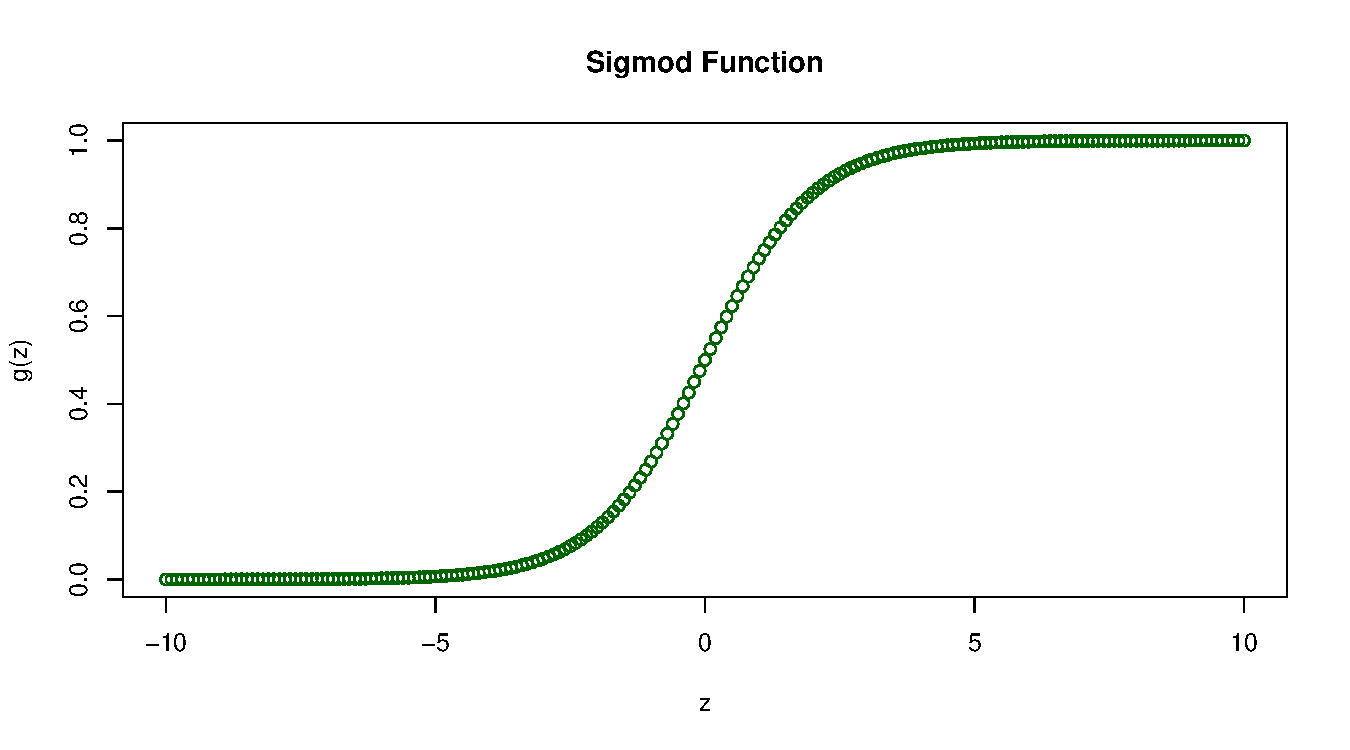
\includegraphics[width=0.9\linewidth]{Images/Prob3-1.pdf}
\end{center}
\bigskip


\qnum{3.2}
The code is in the file \code{Prob3-Commands.R}, part ``Problem 3.2", which calls the file \code{Prob3-Q2.R}, where the actual code lies.
The result is 
\ba 
    \hat\theta
    =& (\hat\theta_0, \hat\theta_1, \cdots, \hat\theta_4)
    = ( -0.993182, -0.02205626, -1.358486, -1.621712, -1.652734 )
\ea 




\qnum{3.3}
We calculate the number of errors, 
\[
    \tx{number of errors} = 
    \sum_{i = 1}^m I(I(x^{(i)}\ge 0.5) = \tx{mpg01}^{(i)}) = 40
\]
where $I(S) = \left\{\begin{aligned}
    1,\quad &\tx{if } S \tx{ is true}\\
    0,\quad &\tx{otherwise}
\end{aligned}\right.$ is the indicator function. $m$ is the number of data points.
Therefore the error rate is 
\[
   \tx{error rate} = \frac{\tx{number of errors}}{m} = 0.1020408
\]
\bigskip


\qnum{3.4}
The scaled values for $x$ is 
\ba 
     (x_1^{\tx{scaled}}, x_2^{\tx{scaled}},x_3^{\tx{scaled}} ,x_4^{\tx{scaled}})
    = (  1.4820530,    1.3912695,    2.4818845,    0.6150391)
\ea 

This is performed by subtracting each feature element by the original feature sample mean, and then dividing each feature element by the original feature sample standard deviation.
Using the formula, the predicted value of mpg01 canbe calculated by
\[
    (1,x_1^{\tx{scaled}},\cdots,x_4^{\tx{scaled}})\hat\theta =  (1,x_1^{\tx{scaled}},\cdots,x_7^{\tx{scaled}})(\hat\theta_0, \hat\theta_1, \hat\theta_2, \cdots, \hat\theta_4)^T
    = 0.0003499786
\]
Since $0.0003499786<0.5$,
\[
    \hat{\tx{mpg01}} = 0
\]

The \code{R} code for the calculation of this question can be found in the Problem 3.4 part of the file \code{Prob3-Commands.R}.
\bigskip


\qnum{3.5}
With $\alpha_1 = 3$, the method quickly blew up, resulting in just 1 iteration.
\begin{center}
    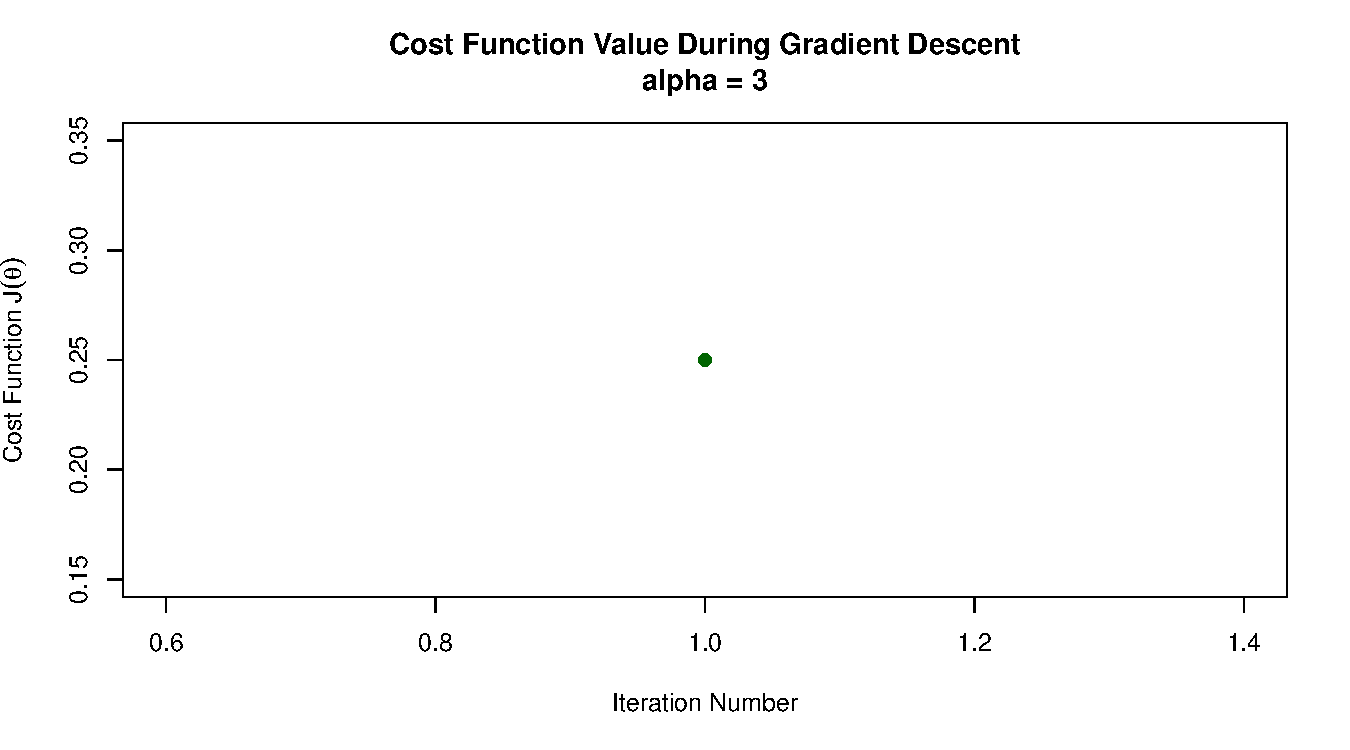
\includegraphics[width=0.9\linewidth]{Images/Prob3-5-alpha1.pdf}
\end{center}

With $\alpha_2 = 0.3$, the method does not seem to converge as the cost function keeps fluctuating. My tolerance on convergence is set to be $1\times 10^{-20}$.
\begin{center}
    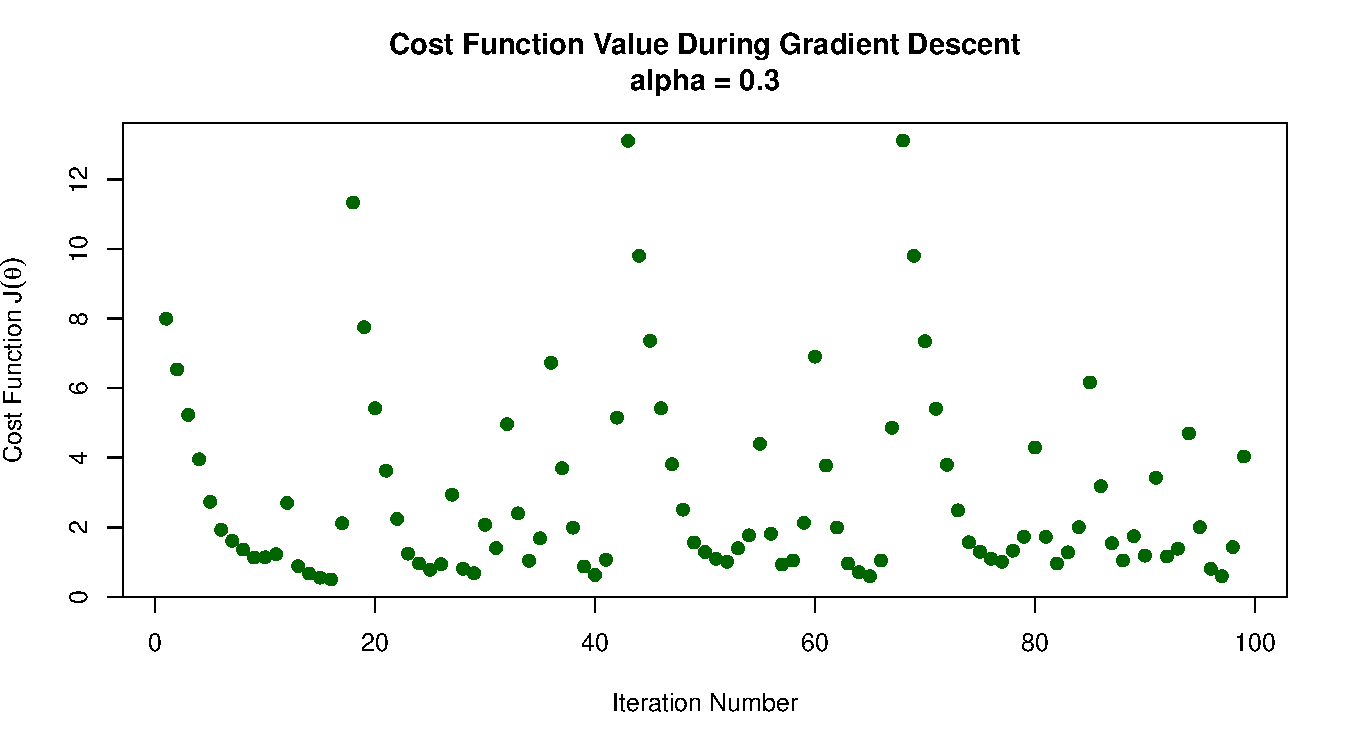
\includegraphics[width=0.9\linewidth]{Images/Prob3-5-alpha2-itr100.pdf}
\end{center}


With $\alpha_3 = 0.03$, the method converges very nicely.
\begin{center}
    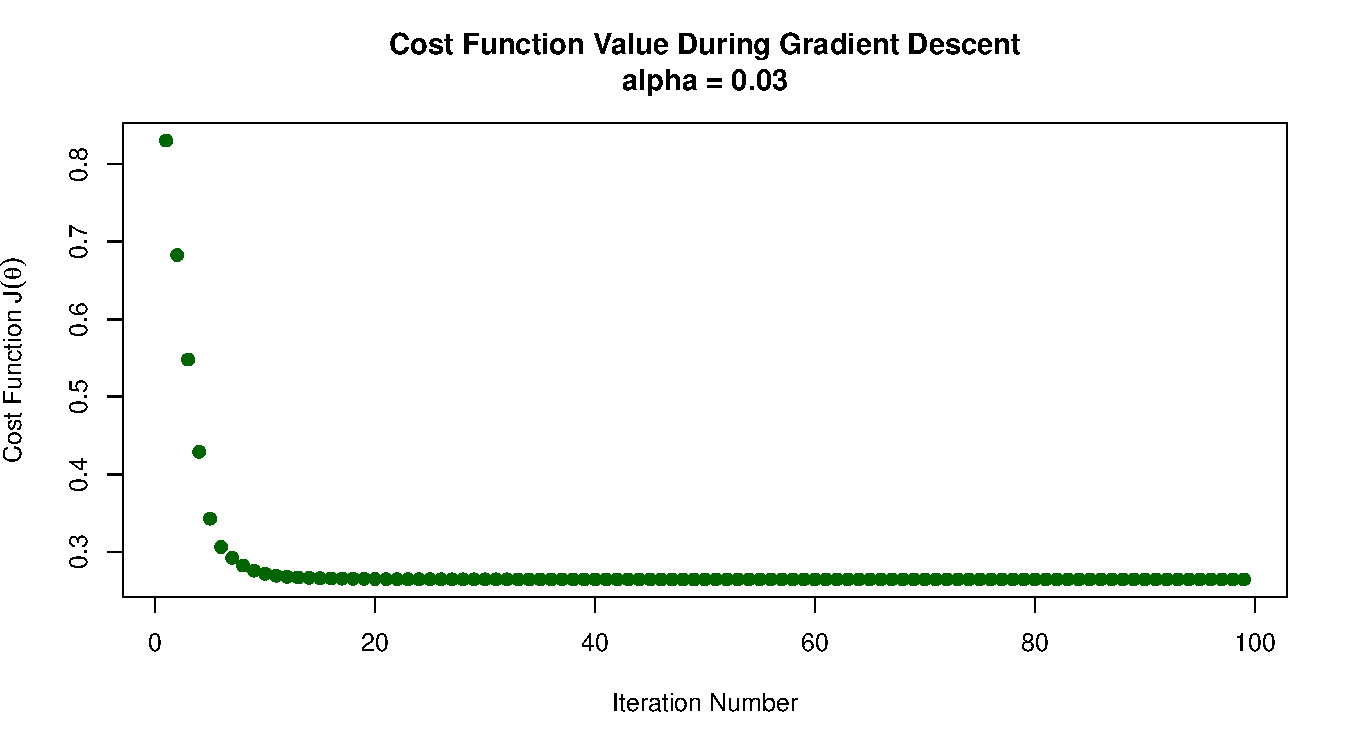
\includegraphics[width=0.9\linewidth]{Images/Prob3-5-alpha3-itr100.pdf}
\end{center}

With $\alpha_4 = 0.00003$, the method converges, but very slowly.
\begin{center}
    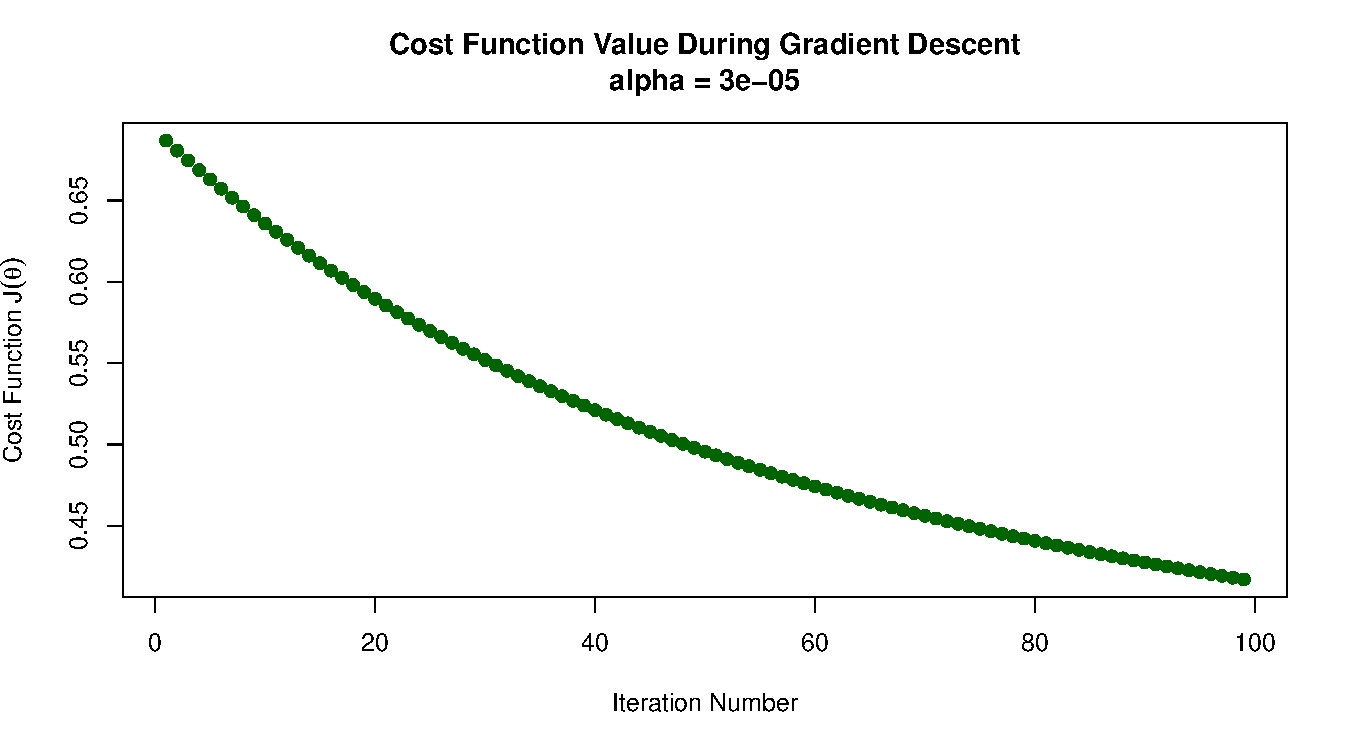
\includegraphics[width=0.9\linewidth]{Images/Prob3-5-alpha4-itr100.pdf}
\end{center}

To illustrate the slow convergence rate for $\alpha_4$, we give a plot for longer run.
\begin{center}
    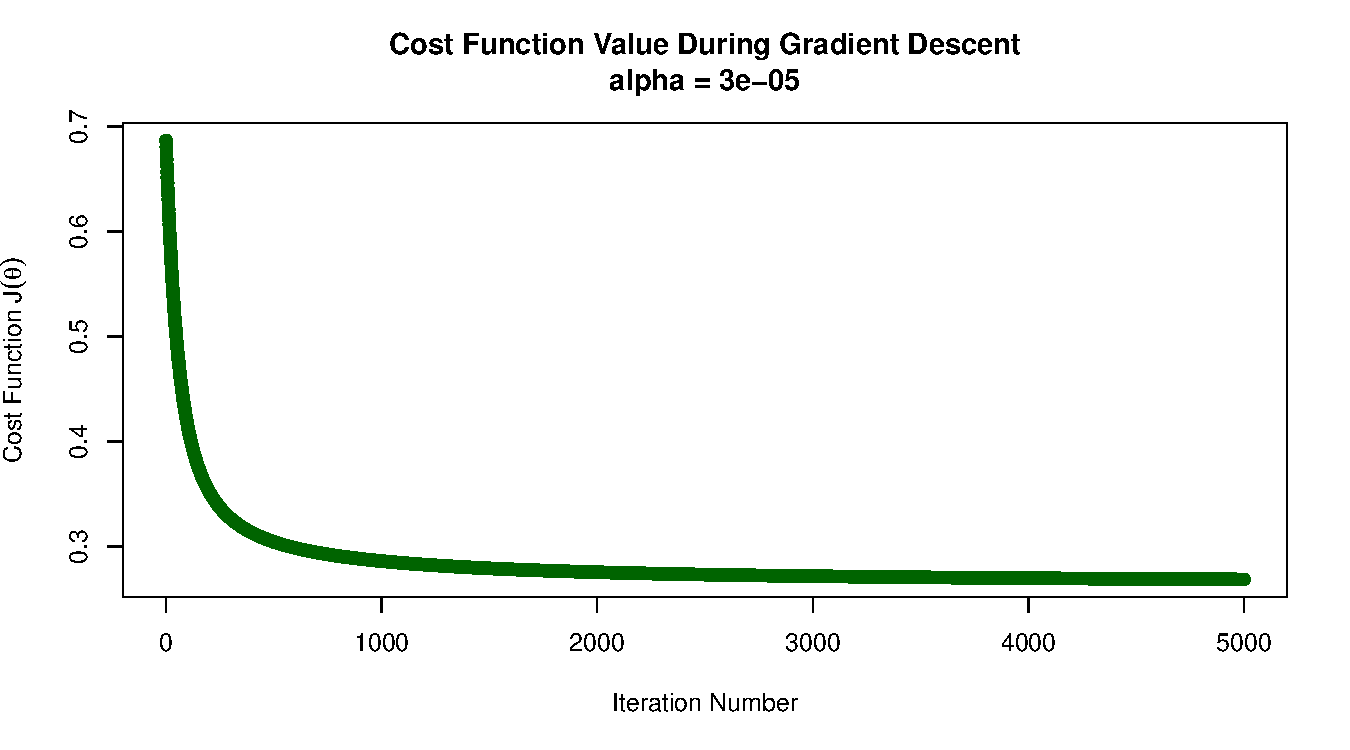
\includegraphics[width=0.9\linewidth]{Images/Prob3-5-alpha4-itr5000.pdf}
\end{center}
Again, we are using very small tolerance $1\times 10^{-20}$, therefore, the method runs a long time for small $\alpha$'s.

In fact, we found that $\alpha = 0.001$ seems to be a very nice choice for learning rate, resulting in convergence at about 30000 iterations.
\bigskip\bigskip




\noindent\textcolor{blue}{\textbf{Summary of Analysis}}
\medskip

As we can see from the plots, when we use $\alpha = 3$, or $0.3$, the method does not converge and the cost function blows up or keeps fluctuating. When $\alpha=0.03$, from the fourth graph, we can see that the method converges very nicely. With $\alpha=0.03$, from the fourth graph, we can see that the method converges but very slowly.  

Therefore, the plots with $\alpha=0.03$ and $0.00003$ look much better than others. And the method converges faster with $\alpha=0.03$.









































%%%%%%%%%%%%%%%%%%%%%%%%%%%%%%%%%%%%%%%%%%%%%%%%%%%%%
       

\newpage
\section*{What to Turn-in -- Submission Instructions}
\begin{itemize}
\item  Zip the files requested below for your submission. The zipped folder should be named as \quotes{usename-section number}, i.e, hakurban-P556
\begin{itemize}
\item The *tex and *pdf of the written answers to this document
\item *\texttt{R}files for:
\begin{itemize}
\item Gradient descent implementation for  problems 1.1 and 1.6 -- file name: \quotes{$linearRegression.R$}.
\item  Normal equation implementation for  problems 1.5 and 1.9  -- file name: \quotes{$normalSolution.R$}.
\item Gradient descent implementation for problem 3.2 -- file name: \quotes{$logisticRegression.R$}.
\item new.Auto data set -- file name: \quotes{$newAuto.R$}.
\end{itemize}
\item A README file that explains how to run your code and other files in the folder
\end{itemize}
\end{itemize}


\end{document}


